\chapter{尼姆游戏与组合博弈} 

\makeatletter
% 核心步骤 A：解除公式与 section 的绑定
% 如果发现公式还在随 section 重置，强制解除它
\@removefromreset{equation}{section}
\@removefromreset{figure}{section}
\@removefromreset{table}{section}

% 核心步骤 B：确保它们只随 chapter 重置
\@addtoreset{equation}{chapter}

% 核心步骤 C：统一编号格式 (章.序号)
\renewcommand{\theequation}{\thechapter.\arabic{equation}}

\makeatother




组合博弈论研究的是具有完美信息(perfect information)的两人博弈，例如跳棋、围棋、国际象棋和尼姆游戏(Nim)。分析这类博弈时，我们主要从规则本身出发，判断在某个局面下，若双方都采用最优策略，谁能够获胜，并进一步衡量一方究竟领先多少。这个领域有一套丰富的数学理论，与离散数学、代数以及本书不展开讨论的计算复杂性理论都有联系，也发展出许多极有想象力的分析方法。

组合博弈并不是经济学中“经典”博弈论的核心内容。不过，它们很好地说明了博弈论真正依赖的是严谨而常常颇不寻常的数学概念，而不是繁复的计算技巧。

本章只是组合博弈的入门。我们先介绍无偏博弈(impartial game)：在任一局面下，两名玩家可选择的行动完全相同。随后我们会证明一个强大而出人意料地简洁的结论(定理\ref{theo:1.14})：每个无偏博弈都等价于某个特定大小的“尼姆堆”(Nim heap)。这一结果由斯普拉格(Sprague，1935)和格伦迪(Grundy，1939)分别独立发现。

在\ref{sec-1.8}节中，我们还会简要介绍更一般的有偏博弈(partizan game)。在这类博弈中，不同玩家的可行动作可能不同，例如一名玩家只能移动白子，另一名玩家只能移动黑子。

本章最后的\ref{sec-1.9}节列出了一些适合继续学习组合博弈的优秀教材。这些教材通常把无偏博弈作为一般组合博弈的特例来处理；本章则反过来，先较为详细地讨论较简单的无偏博弈。

\section{预备知识和学习目标}

本章讨论的组合博弈都是有限博弈。处理这类博弈需要用到数学归纳法，我们会在\ref{sec-1.3}节详细说明。读者如果熟悉自然数上的归纳法，会更容易跟上。阿贝尔群(abelian group)尤其是模 2 加法的知识并非必需，但会有所帮助。我们还假定读者熟悉二进制系统(binary system)：也就是说，数字以 2 为基数书写，只使用 0 和 1，而不是日常使用的十进制数字。

学完本章后，读者应当能够:
\begin{itemize}
\item 以最优策略玩尼姆游戏；
\item 理解选项(option)、博弈之和(game sum)、博弈等价(equivalence)、尼姆值(Nim value)和 MEX 规则等概念；
\item 将这些概念用于分析其他无偏博弈，例如练习中给出的博弈；
\item 理解为什么有些有偏博弈位置可以表示为数，这些数表示左玩家(Left player)安全领先的步数，并理解为什么这些数可能是分母为 2 的幂的分数。
\end{itemize}

\section{尼姆游戏}

组合博弈是具有完美信息的两人胜负博弈：每名玩家都完全知道当前局面，这与桥牌、扑克等含有隐藏信息的纸牌游戏不同。这类博弈没有掷骰子、洗牌之类的随机因素。两名玩家轮流行动，最终必有一方获胜、另一方失败。国际象棋等游戏允许和棋，但本章暂不考虑这种情形。

一个博弈由若干(通常有限个)局面组成，并由规则规定从当前局面可以走到哪些下一局面。规则还要保证博弈最终会结束，也就是迟早会出现某名玩家无法行动的局面。这称为\textit{终止条件}(ending condition)。本章默认采用\textit{正常规则}(normal play)：无法行动的玩家输。与之相对的是\textit{反向规则}(misère play)，即无法行动的玩家赢，也就是最后行动的玩家输。

我们首先研究无偏博弈。在这类博弈中，某个局面下有哪些可行动作并不取决于轮到谁。相反，如果可行动作取决于玩家身份，例如国际象棋中一方只能移动白子、另一方只能移动黑子，这样的博弈称为有偏博弈。

尼姆游戏在无偏博弈中具有核心地位。一个尼姆局面由若干堆代币表示；一次行动就是从某一堆中取走若干枚代币，至少取一枚，也可以取完整堆。在正常规则下，最后还能行动的玩家获胜。

先看尼姆局面$(1,2,3)$：这里有 3 个尼姆堆，大小分别为 1、2 和 3。一个合法行动是从大小为 3 的堆中取走 2 枚代币，如下图所示:

\begin{figure}[htbp]
  \centering
  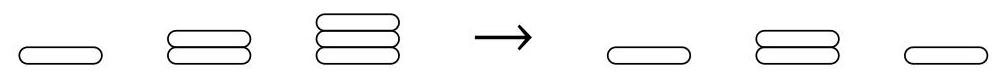
\includegraphics[width=0.75\linewidth]{images/inline-1-nim-move.jpg}
\end{figure}



我们把这一步记作从$(1,2,3)$走到$(1,2,1)$。由于玩家可以在任意一堆上行动，堆的排列顺序没有意义，所以$(1,2,1)$也可以写成$(1,1,2)$。一个局面的\textit{选项}，是指当前玩家通过一步合法行动能够到达的局面。下面用向下的线表示这些行动:
\begin{equation}
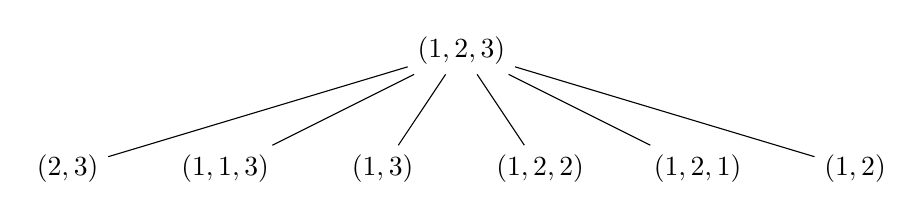
\begin{tikzpicture}[level distance=1.5cm,
  level 1/.style={sibling distance=2cm},
  baseline=(current bounding box.center)]
  % 根节点
  \node {$(1,2,3)$}
    child {node {$(2,3)$}}
    child {node {$(1,1,3)$}}
    child {node {$(1,3)$}}
    child {node {$(1,2,2)$}}
    child {node {$(1,2,1)$}}
    child {node {$(1,2)$}};
\end{tikzpicture}
\label{eq:1.1}
\end{equation}
 

其中，第一个选项$(2,3)$是从$(1,2,3)$中取走整个大小为 1 的堆得到的；第二个选项$(1,1,3)$是从大小为 2 的堆中取走 1 枚代币得到的；其余选项依此类推。如果继续把所有可能行动一直画到游戏结束，就得到一棵\textit{博弈树}(game tree，第 4 章会更系统地讨论博弈树)。显然相同的选项可以合并，例如从$(1,2,2)$走到的$(1,1,2)$和$(1,2,1)$表示同一局面。不过，来自不同前驱的行动不会合并到同一个节点。比如$(1,1,2)$既可以由$(1,1,3)$得到，也可以由$(1,2,2)$得到，但在博弈树中它会出现两次。这样，每个节点都对应唯一的一段行动历史(history of moves)。

在无偏博弈中，当前局面的合法行动与轮到哪名玩家无关。因此，每个局面都恰好属于两类之一：\textit{必胜位置}(winning position)或\textit{必败位置}(losing position)。这里的“必胜”和“必败”都是相对于当前行动者而言，并且假设双方之后都采用最优策略。必胜位置意味着当前玩家存在一步制胜行动(winning move)，并能在随后的局面中继续维持胜势；必败位置则意味着当前玩家无论怎么走，都会把对手送入必胜位置，从而最终输掉游戏。

如果把局面 $(1,2,3)$之后所有可能的行动都画出来，博弈树已经相当庞大。不过，只要用到下面关于至多两堆尼姆游戏的简单观察，就可以直接从\eqref{eq:1.1}的选项判断出 $(1,2,3)$ 是一个必败位置:
如果把局面$(1,2,3)$之后所有可能的行动都画出来，博弈树已经相当庞大。不过，只要用到下面关于至多两堆尼姆游戏的简单观察，就可以直接从\eqref{eq:1.1}的选项判断出$(1,2,3)$是一个必败位置:
\begin{itemize}
\item 没有尼姆堆时，根据正常规则，这是一个必败位置。
\item 只有一堆时，这是一个必胜位置；制胜行动是取走整堆。
\item 有两堆时，当且仅当两堆大小不同才是必胜位置。制胜行动是把较大的堆减小到与较小的堆相同，从而把对手送入两个等大堆构成的必败位置。若两堆原本就相等，那么当前玩家的任何行动都会使两堆变得不等，也就是把对手送入必胜位置；因此，两个等大堆构成必败位置。
\end{itemize}

式\eqref{eq:1.1}中 $(1,2,3)$ 的每个选项都是必胜位置，因为从每个选项出发，都能再走到两个等大堆构成的必败位置，如下所示:
式\eqref{eq:1.1}中$(1,2,3)$的每个选项都是必胜位置，因为从每个选项出发，都能再走到两个等大堆构成的必败位置，如下所示:
\begin{equation}
\begin{adjustbox}{width=0.8\textwidth, keepaspectratio}
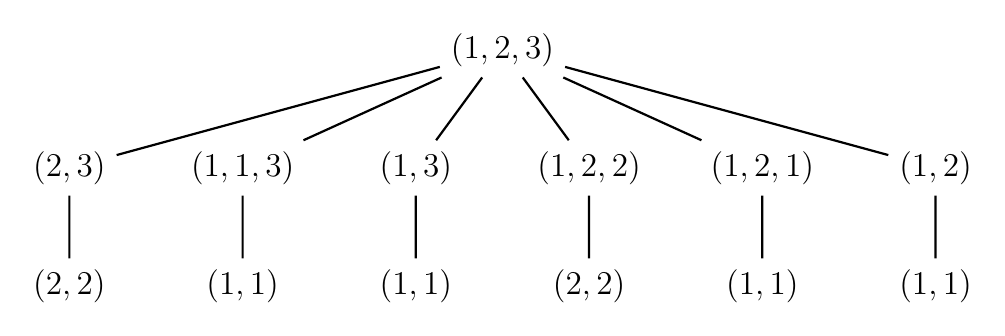
\begin{tikzpicture}[
    line width=0.8pt, % 统一设置所有线条宽度
    level distance=1.5cm, % 稍微增加层距，视觉上更舒展
    level 1/.style={sibling distance=2.2cm},
    level 2/.style={sibling distance=1cm},
    baseline=(current bounding box.center),
   every node/.style={
        inner sep=2pt,      % 增加内部间距，让线离数字更远
        outer sep=2pt,      % 增加外部间距，进一步推开连线
        font=\large
    }
]
  % 根节点
  \node {$(1,2,3)$}
    child { node {$(2,3)$} 
        child { node {$(2,2)$} } 
    }
    child { node {$(1,1,3)$} 
        child { node {$(1,1)$} }
    }
    child { node {$(1,3)$} 
        child { node {$(1,1)$} }
    }
    child { node {$(1,2,2)$} 
        child { node {$(2,2)$} }
    }
    child { node {$(1,2,1)$} 
        child { node {$(1,1)$} }
    }
    child { node {$(1,2)$} 
        child { node {$(1,1)$} }
    };
\end{tikzpicture}
\end{adjustbox}
  \label{eq:1.2}
\end{equation}

这张图只展示了从$(1,2,3)$出发的部分两步行动序列，因此并不是完整博弈树的顶部。图中完整列出了从初始局面$(1,2,3)$出发的所有第一步行动；至于第二步，则每个分支只画出一种会走向必败位置的制胜行动。


\begin{lemma}\label{lem:1.1}
在无偏博弈中，一个博弈位置是必败位置当且仅当它的所有选项都是必胜位置。一个博弈位置是必胜位置当且仅当它的至少一个选项是必败位置；移动到该必败位置的行动就是一个必胜行动。
\end{lemma}

这个引理同样适用于没有任何选项的局面：在“空真”的意义下，它的所有选项都是必胜的，因为根本没有选项，所以该局面是必败位置。事实上，这个引理也可以看作必胜、必败位置的定义。它不是循环定义，而是\textit{递归}(recursive)定义，因为一个局面的选项总是在某种意义上更接近游戏结束，也就是更\textit{简单}。\ref{sec-1.3}节会把这一点说清楚，并给出引理\ref{lem:1.1}的正式证明。

必胜位置和必败位置都建立在双方最优行动的假设之上。宾莫尔(2007 年，第 49 页)写道：“一部名为《去年在马里昂巴德》的沉闷艺术电影，大部分内容是角色们非常糟糕地玩尼姆游戏。”在这部 1961 年上映、由阿伦·雷乃执导的电影中，角色多次玩反向尼姆游戏，起始局面总是 $(1,3,5,7)$。某个场景中，连续出现了三个局面:

\[
(2,3,6) \xrightarrow{\text{player I}}( 2,3,5) \xrightarrow{\text{player II}} (2,3,1)
\]

随后轮到玩家 I 行动，而玩家 I 最终输了。由此可见，他确实下得很糟。原因是：如果 $(2,3,1)$ 是必胜位置，那么玩家 I 没有把胜利把握住；如果 2,3,1 是必败位置(事实上正是如此)，那么玩家 I 本应从 2,3,6 直接走到这个局面，却错过了这一步。
必胜位置和必败位置都建立在双方最优行动的假设之上。宾莫尔(2007 年，第 49 页)写道：“一部名为《去年在马里昂巴德》的沉闷艺术电影，大部分内容是角色们非常糟糕地玩尼姆游戏。”在这部 1961 年上映、由阿伦·雷乃执导的电影中，角色多次玩反向尼姆游戏，起始局面总是$(1,3,5,7)$。某个场景中，连续出现了三个局面:

\[
(2,3,6) \xrightarrow{\text{player I}} (2,3,5) \xrightarrow{\text{player II}} (2,3,1)
\]

随后轮到玩家 I 行动，而玩家 I 最终输了。由此可见，他确实下得很糟。原因是：如果$(2,3,1)$是必胜位置，那么玩家 I 没有把胜利把握住；如果$(2,3,1)$是必败位置(事实上正是如此)，那么玩家 I 本应从$(2,3,6)$直接走到这个局面，却错过了这一步。

另一方面，正因为人们不知道一个博弈的最优玩法，它才往往更有趣。以国际象棋为例，那里允许和棋。类似引理~\ref{lem:1.1} 的论证可以说明：要么白方能确保获胜，要么黑方能确保获胜，要么双方都能确保和棋。但从“最优玩法究竟会导向哪种结果”这个意义上说，国际象棋尚未被解决。也正因为玩家并不能完美行动，它仍然是一个有趣的游戏。

相比之下，尼姆游戏已经由布顿(1901)完全解决。下面用一个已经相当棘手的尼姆局面$(4,5,9,14)$来展示他的必胜策略；这个局面是必胜位置。

 

\begin{figure}[htbp]
  \centering
  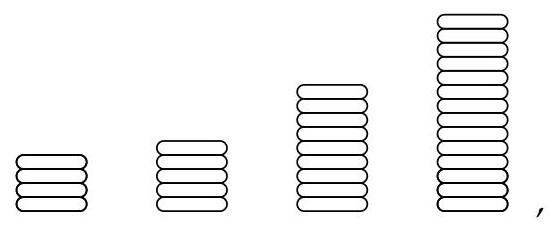
\includegraphics[width=0.6\linewidth]{images/inline-1-bouton-nim-position.jpg}
\end{figure}


关键是把各个尼姆堆的大小写成\textit{二进制}。下表说明，一个制胜行动是把大小为 5 的堆减小到 3，从而得到必败位置$(4,3,9,14)$:

\begin{equation}
    \adjustbox{valign=c}{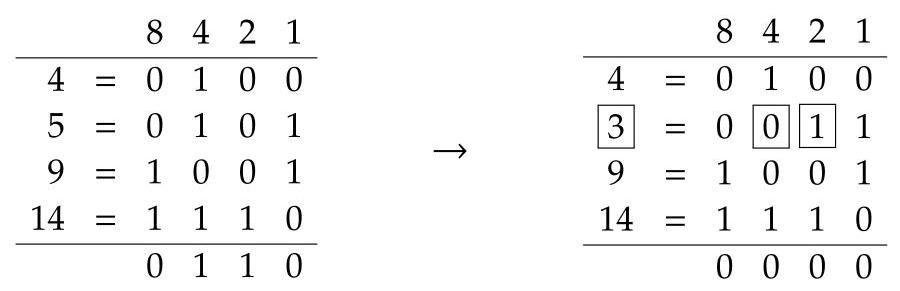
\includegraphics[width=0.7\textwidth]{images/eq-1-3-binary-nim.jpg}}
     \label{eq:1.3}
\end{equation}


在\eqref{eq:1.3}中，最上面一行列出用二进制表示堆大小时涉及的 2 的幂。例如，$5 = 0 \cdot 8 + 1 \cdot 4 + 0 \cdot 2 + 1 \cdot 1$。最下面一行称为这些堆大小的尼姆和(Nim sum)，它是逐列做“无进位的模 2 加法”得到的：某一列中 1 的个数为偶数时，该列尼姆和为 0；为奇数时，该列尼姆和为 1。

我们断言，一个尼姆局面是必败位置，当且仅当每一列的尼姆和都为 0，就像\eqref{eq:1.3}右侧那样。这样的局面称为零位置。根据引理~\ref{lem:1.1}，要证明这一点，只需证明:

 
(a) 从零位置出发的任何一步都会到达非零位置，因此到达必胜位置；并且

(b) 从每个非零位置出发，都存在一步行动可以到达零位置。

先看 (a)，这很直接：一步行动只改变一个尼姆堆，也就是只改变二进制表中的一行，并且至少会改变该堆二进制表示中的一位。因此，对应列的尼姆和也会改变，结果不可能仍然全为 0。

条件 (b) 则是在非零位置中找到一步制胜行动，例如\eqref{eq:1.3}左侧的局面。做法如下:

\begin{itemize}
\item 找出尼姆和中最左边的“1”列。该列一定存在，因为当前并不是零位置。它对应于尼姆和二进制表示中最高的 2 的幂；在这里是 \(4 = {2}^{2}\)。
\item 按定义，必有奇数个尼姆堆在这一列上为 1。在\eqref{eq:1.3}中，它们分别是大小为 4、5 和 14 的堆。任选其中一行；这里选择大小为 5 的堆。
\item 在所选行中，把尼姆和中为 1 的那些列逐一“翻转”。在本例中，就是第 4 列和第 2 列；\eqref{eq:1.3}右侧方框标出了这些改动。被改动的最高位原来是 1，现在变成 0。即使后面的较低位全都从 0 变成 1，得到的整数仍然比原来小(也可能变成 0，这意味着取走整堆)。因此，制胜行动就是把这一堆减小到那个新数；本例中是从 5 减小到 3。
\end{itemize}

经过这些步骤，原来尼姆和为 1 的列会全部变成 0，而原来为 0 的列保持为 0。于是新的尼姆和每一列都是 0，得到的局面正是零位置，这就证明了 (b)。

尼姆游戏的这套制胜策略可以用纸笔完成，但实际对局时未必容易心算。对于较小的堆，一个有用的直观图像是把每堆代币(这里用点表示)按不同的 2 的幂分组:


\begin{equation}
    \adjustbox{valign=c}{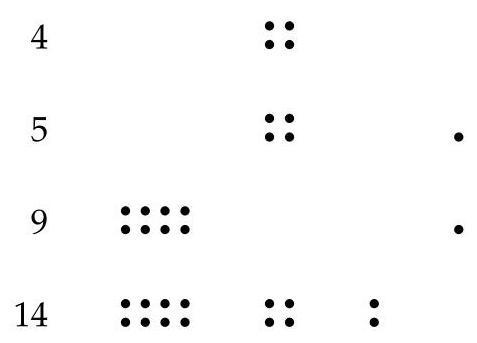
\includegraphics[width=0.5\textwidth]{images/eq-1-4-dot-binary-nim.jpg}}
     \label{eq:1.4}
\end{equation}


这与\eqref{eq:1.3}左侧的表格等价，只是不再显式写出二进制位。图中可以看出，出现奇数次的 2 的幂是 4 和 2。制胜行动必须改变某一堆，使这些幂次之后都出现偶数次。比如，把大小为 5 的堆中的四个点改成两个点，即 \( \twodots \twodots \rightarrow   \twodots\)，就对应于\eqref{eq:1.3}中从大小为 5 的堆取走两个代币。同样的制胜行动也可以在大小为 4 的堆上完成。第三种制胜行动是从大小为 14 的堆中取走六个代币(\(\twodots\twodots \text{ 和 }  \twodots\))。注意，改变后的堆仍必须由互不相同的 2 的幂组成。在大小为 14 的堆中，不能把 \( \twodots \twodots\) 简单改成 \(\twodots\)，因为预期结果 $ \twodots \twodots \twodots \twodots\quad\twodots\quad\twodots $ 不是合法的二进制分解，其中 2 出现了两次。事实上，从大小为 14 的堆中只取走两个代币会得到 $ \twodots\twodots\twodots\twodots\quad\twodots\twodots$，整个尼姆局面并不是零位置。一旦选定要操作的堆，需要取走多少代币就是唯一确定的。

\section{自上而下归纳}\label{sec-1.3}

讨论组合博弈时，为了行文简洁，我们常用“博弈”来指“博弈位置”(game position)。每个博弈 \(G\) 都有有限个选项 \({G}_{1},\ldots ,{G}_{m}\)，也就是从 \(G\) 出发一步可以到达的局面，如图所示:
 
\begin{equation}
    \adjustbox{valign=c}{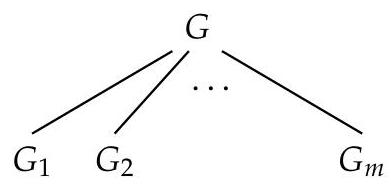
\includegraphics[width=0.5\textwidth]{images/eq-1-5-game-options.jpg}}
     \label{eq:1.5}
\end{equation}


如果 \(m = 0\)，则 \(G\) 没有选项。我们用 0 表示没有选项的博弈；按照正常规则(normal play)，它是必败位置。若 \(G\) 有选项，那么这些选项本身也是博弈，并继续由它们各自的选项定义。这样，任一博弈都可以完全由它的选项递归刻画。换句话说，起始局面就决定了整个博弈。

下面为博弈引入一种特别适用的归纳法。它不是沿着自然数一步步往前推，而是作用在一个偏序(partial order)上，相关概念见下面的背景材料。
\begin{mybox}{背景材料：偏序}
     
 
\begin{definition}[偏序、全序]\label{def:1.2}集合 \(S\) 上的二元关系 \(\leq\)，若对 \(S\) 中任意 \(x,y,z\) 都满足以下条件，则称为\textit{偏序}(partial order):

\(\leq\) 的传递性(transitive): \(x \leq  y\) 且 \(y \leq  z \Rightarrow  x \leq  z\);

\(\leq\) 的自反性(reflexive): \(x \leq  x\);

\(\leq\) 的反对称性(antisymmetric): \(x \leq  y\) 且 \(y \leq  x \Rightarrow  x = y\) 。

此外，如果对 \(S\) 中任意 \(x,y\)，总有 \(x \leq y\) 或 \(y \leq x\)(即 \(\leq\) 是完备的)，则称 \(\leq\) 为\textit{全序}(total order)。
\end{definition}


给定偏序 \(\leq\) 后，若 \(x \leq y\)，我们通常说“\(x\) 小于等于 \(y\)”。相应地，严格关系 \(x < y\)(即“\(x\) 小于 \(y\)”)定义为:

\begin{equation}\label{eq:1.6}
x < y\; \Leftrightarrow  \;x \leq  y\;\text{ and }\;x \neq  y. 
\end{equation}

关系 \(<\) 称为与 \(\leq\) 对应的严格序(strict order)。练习~\ref{exer:1.1}要求你反过来证明：如果集合 \(S\) 上的关系 \(<\) 满足合适性质(传递性和非自反性)，就可以由它定义一个偏序 \(\leq\)。定义方式为

\begin{equation}\label{eq:1.7}
x \leq  y\; \Leftrightarrow  \;x < y\;\text{ or }\;x = y. 
\end{equation}

如果 \(S\) 中不存在 \(y\) 满足 \(y < x\) ，则 \(S\) 中的元素 \(x\) 称为\textit{极小元}(minimal element)。

任何有理数集或实数集 \(S\) 都带有熟悉的 \(\leq\) 关系，而且它是全序。另一个最重要、但通常不是全序的偏序，是集合族 \(S\) 上的包含关系(set inclusion) \(\subseteq\)。在这种情形下，定义~\ref{def:1.2}中的元素 \(x,y\) 通常写作大写字母 \(A,B\)。若 \(A\) 是 \(B\) 的子集(允许 \(A=B\))，就写作 \(A \subseteq B\)。包含序一般不是全序，因为两个集合可能不可比较，也就是 \(A \subseteq B\) 和 \(B \subseteq A\) 都不成立。例如 \(A=\{1,2\}\) 且 \(B=\{2,3,4\}\) 时就是如此。若 \(S\) 是有限集 \(\{1,\ldots,n\}\) 的所有子集组成的集合，则在包含序下，\(S\) 有唯一极小元，即空集 \(\varnothing\)。若 \(S\) 只包含 \(\{1,\ldots,n\}\) 的非空子集，则极小元是各个单元素集 \(\{1\},\{2\},\ldots,\{n\}\)。

\end{mybox}

考虑一个博弈集合 \(S\)。例如，\(S\) 可以由某个起始局面以及从它出发经过任意行动序列能够到达的所有局面组成。对 \(S\) 中两个博弈 \(G\) 和 \(H\)，若存在一串行动能从 \(G\) 到达 \(H\)，就称 \(H\) 比 \(G\) 更简单。这里允许 \(G=H\)，对应空的行动序列。“更简单”关系给出一个偏序，下面仍记为 \(\leq\)。注意，\(\leq\) 是反对称的，因为若存在非空行动序列能从 \(G\) 回到 \(G\)，就会违反终止条件。终止条件等价地带来以下性质:

\begin{equation}
\text{$S$ 的每个非空子集都有一个极小元。}\label{eq:1.8}
\end{equation}

若 \(S\) 有某个非空子集 \(T\) 没有极小元，就可以构造出一个无限对局：从 \(T\) 中任取一个 \(G\) 开始。由于 \(G\) 不是极小元，\(T\) 中存在某个 \(H\) 满足 \(H<G\)，因此可以从 \(G\) 经过若干步到达 \(H\)。同理，\(H\) 也不是极小元，又可以从 \(H\) 到达 \(T\) 中更简单的某个局面。如此不断继续，就得到一条无限行动序列，这与终止条件矛盾。
 
对于任何具有性质\eqref{eq:1.8}的偏序，以下定理成立。

\begin{theorem}\label{theo:1.3}设集合 \(S\) 带有偏序 \(\leq\)，并且该偏序满足\eqref{eq:1.8}。令 \(P(x)\) 是关于 \(S\) 中元素 \(x\) 的一个命题。若对每个 \(x\in S\)，只要所有 \(y<x\) 都满足 \(P(y)\)，就能推出 \(P(x)\)，那么 \(P(x)\) 对 \(S\) 中所有 \(x\) 都成立。用符号表示，其中“\(\forall x\)”表示“对 \(S\) 中所有元素 \(x\)”:

\begin{equation}
\left( {\forall x : \left( {\forall y < x : P\left( y\right) }\right)  \Rightarrow  P\left( x\right) }\right)  \Rightarrow  \left( {\forall x : P\left( x\right) }\right).  \label{eq:1.9}
\end{equation}
\end{theorem}

\begin{proof}
按定理假设，对任意 \(x\)，只要所有满足 \(y<x\) 的元素 \(y\) 都使 \(P(y)\) 成立，就有 \(P(x)\) 成立。考虑集合 \(T=\{z\in S\mid P(z)\text{ 为假}\}\)。若 \(T\) 为空，则结论已经成立。反设 \(T\) 非空。由\eqref{eq:1.8}，\(T\) 有一个极小元 \(x\)。那么所有满足 \(y<x\) 的元素 \(y\) 都不在 \(T\) 中，因此 \(P(y)\) 为真。由假设\eqref{eq:1.9}可得 \(P(x)\) 也为真，这与 \(x\in T\) 矛盾。因此 \(T\) 必为空集。
\end{proof}


定理~\ref{theo:1.3}给出了一种\textit{归纳方法}：只要能从所有更小元素 \(y<x\) 满足 \(P(y)\) 推出 \(P(x)\)，并且偏序满足\eqref{eq:1.8}，就能推出所有元素都满足 \(P\)。一个经典应用是证明质数分解定理：若整数 \(x\geq 2\)，则 \(x\) 可以写成若干质数的乘积。证明时先说明 \(x\) 有一个质因数 \(p\)。要么 \(x=p\)，此时结论立即成立；要么存在整数 \(y\) 满足 \(2\leq y<x\) 且 \(x=p\cdot y\)\footnote{译者注：可以证明，每个 $x\ge2$的整数要么本身是质数，要么有一个质数 $p\mid x$。}。后一种情况下，由归纳假设，若 \(P(y)\) 为真，则 \(y=p_{1}p_{2}\cdots p_{k}\)，其中 \(p_{1},p_{2},\ldots,p_{k}\) 都是质数。因此 \(x=pp_{1}p_{2}\cdots p_{k}\)，从而 \(P(x)\) 成立。因为任何非空正整数集合都有极小元，所以可以应用定理~\ref{theo:1.3}。

这种方法称为“自上而下”归纳法(top-down induction)，因为论证从“顶部”的元素 \(x\) 出发，再调用所有更小元素 \(y<x\) 的性质 \(P(y)\)。在实际证明中，我们遇到 \(y\) 时往往并不知道它比 \(x\) 小多少，质数分解的证明就是这样。相比之下，自然数上的普通归纳法通常先证明 \(P(1)\)，再一步一步证明 \(P(n)\Rightarrow P(n+1)\)。自上而下归纳法更强：在自然数全序上它就是常说的强归纳法，而在偏序上也同样适用。

普通归纳证明中通常需要单独处理的基础情形到哪里去了？基础情形是说，对任意极小元 \(x\)，\(P(x)\) 成立(若 \(\leq\) 是全序，则通常只有一个极小元)。答案是：基础情形已经包含在\eqref{eq:1.9}的假设中。式\eqref{eq:1.9}左侧要求

\begin{equation}
\left( {\forall y < x : P\left( y\right) }\right)  \Rightarrow  P\left( x\right) \label{eq:1.10}
\end{equation}

对所有 \(x\) 成立，当然也要对极小元成立。而当 \(x\) 是极小元时，并不存在 \(y<x\)，所以 \(\left( {\forall y < x : P\left( y\right) }\right)\) 在空真意义下成立。因此，\eqref{eq:1.10}迫使 \(P(x)\) 成立；这正是基础情形。

作为证明技巧，我们通常可以直接使用定理~\ref{theo:1.3}，不必每次都把极小元单独拿出来讨论。它还允许我们在研究一个博弈时，递归地调用更简单博弈已经满足的同一性质。

现在用自上而下归纳法证明引理~\ref{lem:1.1}。也就是说，任意博弈 \(G\) 要么是必胜位置，要么是必败位置。假设所有比 \(G\) 更简单的博弈都已经如此，特别是 \(G\) 的所有选项。如果 \(G\) 的所有选项都是必胜位置，那么当前玩家无论怎么走，都会让对手进入必胜位置，因此 \(G\) 是必败位置。如果 \(G\) 的选项并非全是必胜位置，那么其中某个选项 \(H\) 是必败位置；当前玩家走到 \(H\) 后即可确保获胜，所以 \(G\) 是必胜位置。这个论证并不比前面的直观说明更深；定理~\ref{theo:1.3}只是保证它在形式上是严谨的。

\section{ 博弈之和与博弈等价性}

组合博弈常常可以分解为若干彼此独立的部分；玩家每一步要决定在哪一部分中行动。这正是“博弈之和”这一概念要刻画的内容。

\begin{definition}\label{def:1.4} 假设 \(G\) 和 \(H\) 是博弈位置，它们的选项(通过一步行动到达的位置)分别是 \({G}_{1},\ldots ,{G}_{k}\) 和 \({H}_{1},\ldots ,{H}_{m}\) 。那么博弈之和 \(G + H\) 的选项是

\begin{equation}
{G}_{1} + H,\ldots ,{G}_{k} + H,\quad\quad G + {H}_{1},\ldots ,G + {H}_{m}.  \label{eq:1.11}
\end{equation}
\end{definition}
 \eqref{eq:1.11}中的第一组选项 \({G}_{1} + H,\ldots ,{G}_{k} + H\) 表示玩家在 \(G\) 中行动；第二组选项 \(G + {H}_{1},\ldots ,G + {H}_{m}\) 表示玩家在 \(H\) 中行动。无论在哪一部分行动，另一部分都保持不变。例如，一个尼姆局面就是若干尼姆堆的博弈之和，因为玩家每次只能在其中一堆中取子。

定义 \ref{def:1.4}是一个递归定义，因为博弈之和是根据其选项来定义的，而这些选项本身也是博弈之和(但它们是更简单的博弈)。

进一步地，若在恰当限定的博弈集合上考察该运算，博弈之和构成一个阿贝尔群：运算交换、结合，并存在单位元与逆元。具体地，对任意博弈 $G,H,J$，有

\begin{equation}
G + H = H + G\;\text{ 和 }\;\left( {G + H}\right)  + J = G + \left( {H + J}\right). \label{eq:1.12}
\end{equation}

交换律成立，是因为\eqref{eq:1.11}中选项的排列顺序并不重要。结合律也成立，因为 \(\left( {G + H}\right)+J\) 和 \(G+\left( {H+J}\right)\) 本质上都表示：玩家在 \(G,H,J\) 三个分量中选一个行动，其余两个分量保持不变。因此，我们可以直接使用等式\eqref{eq:1.12}。更一般地，在若干博弈 \({G}_{1},\ldots,{G}_{n}\) 的和中，玩家每步恰好只在其中一个博弈中行动，与这些博弈如何排列无关，所以可以不加括号地写作 \({G}_{1}+\cdots+{G}_{n}\)。

没有选项的必败博弈 0 是博弈之和的零元(中性元素)：对任意博弈 \(G\)，都有 \(G+0=G\)，因为把 0 加到 \(G\) 上不会提供任何额外行动。

若要得到群结构，每个博弈 \(G\) 都需要有一个“负”博弈 \(-G\)，使 \(G+\left({-G}\right)=0\)。不过，只要 \(G\) 有选项，这个等式就不能按字面成立，因为 \(G+\left({-G}\right)\) 也会有选项，而 0 没有选项。因此，我们需要更弱、更合适的条件:

\begin{equation}
G + \left( {-G}\right)  \equiv  0, \label{eq:1.13} 
\end{equation}

其中 \(G \equiv  H\) 表示根据以下定义，两个博弈 \(G\) 和 \(H\) 是等价的。
\begin{definition}\label{def:1.5}
两个博弈 \(G,H\) 称为等价，记为 \(G \equiv H\)，当且仅当对任意其他博弈 \(J\)，博弈之和 \(G+J\) 是必败位置当且仅当 \(H+J\) 是必败位置。 \end{definition}

\begin{lemma}\label{lem:1.6}
定义~\ref{def:1.5}中的关系 \(\equiv\) 确实是博弈之间的等价关系，即它满足自反性、对称性和传递性。
\end{lemma}
\begin{proof}
自反性意味着对于任何博弈 \(G\) 有 \(G \equiv  G\) ，这显然成立。对称性意味着如果 \(G \equiv  H\) 则 \(H \equiv  G\) ，这也根据定义成立。假设对于博弈 \(G,H,K\) 有 \(G \equiv  H\) 和 \(H \equiv  K\) 。传递性意味着 \(G \equiv  K\) 。考虑任何其他博弈 \(J\) 。如果 \(G + J\) 是必败的，那么由于 \(G \equiv  H\) ， \(H + J\) 是必败的，又因为 \(H \equiv  K\) ， \(K + J\) 是必败的。反之，如果 \(K + J\) 是必败的，那么由于 \(H \equiv  K\) ， \(H + J\) 是必败的，再由于 \(G \equiv  H\) ， \(G + J\) 是必败的。因此， \(G + J\) 是必败的当且仅当 \(K + J\) 是必败的，即 \(G \equiv  K\) 。这表明 \(\equiv\) 是传递的。
\end{proof}


在定义~\ref{def:1.5}中取 \(J=0\) 可知，若 \(G\) 和 \(H\) 等价，则它们要么同为必败位置，要么同为必胜位置。更重要的是，等价不仅要求 \(G\) 和 \(H\) 本身结果相同，还要求把任意博弈 \(J\) 加到它们上面后，\(G+J\) 与 \(H+J\) 的结果仍然相同。这比单纯属于同一结果类强得多。例如，两个不同大小的尼姆堆都是必胜位置，但并不等价。我们把这一点表述为下面的引理。

\begin{lemma}\label{lem:1.7}两个尼姆堆等价当且仅当它们的大小相等。\end{lemma}

证明:设 \(G\) 和 \(H\) 是两个大小不同的尼姆堆，并在定义~\ref{def:1.5}中取 \(J=G\)。回忆一下，两个尼姆堆大小不同时是必胜位置，大小相同时是必败位置。因此 \(G+G\) 是必败位置，而 \(H+G\) 是必胜位置，所以 \(G\) 与 \(H\) 不等价。若 \(G\) 和 \(H\) 大小相同，它们就是同一个博弈，当然等价。

另一方面，任意两个必败博弈都是等价的，因为它们都等价于没有选项的博弈 0。
\begin{lemma}\label{lem:1.8}
\(G\) 是必败位置当且仅当 \(G \equiv  0\) 。
\end{lemma}
\begin{proof}
若 \(G \equiv 0\)，则在定义~\ref{def:1.5}中取 \(J=0\)。由于 0 是必败位置，\(G\) 也必败。因此只需证明“仅当”部分。

设 \(G\) 是必败位置。我们要证明 \(G \equiv 0\)，也就是对任意其他博弈 \(J\)，\(G+J\) 必败当且仅当 \(0+J\) 必败。由于 \(0+J=J\)，这等价于下面两个蕴含关系:

\begin{equation}
G + J\text{ 是必败的 } \Rightarrow  J\text{ 是必败的 }  \label{eq:1.14}
\end{equation}

并且(为了对称，我们添加假设 \(G\) 是必败位置)

\begin{equation}
G\text{ 和 }J\text{ 都是必败的 } \Rightarrow  G + J\text{ 是必败的. }  \label{eq:1.15}
\end{equation}

条件\eqref{eq:1.15}很直观：如果 \(G\) 和 \(J\) 都是必败位置，那么在 \(G+J\) 中也没有制胜办法，因为后手总能在相应分量中作出回应。下面用自上而下归纳给出正式证明。设 \(G\) 和 \(J\) 都必败。要证明 \(G+J\) 必败，只需证明它的每个选项都是必胜位置。任一选项要么形如 \({G}^{\prime}+J\)，其中 \({G}^{\prime}\) 是 \(G\) 的一个选项；要么形如 \(G+{J}^{\prime}\)，其中 \({J}^{\prime}\) 是 \(J\) 的一个选项。先看 \({G}^{\prime}+J\)。因为 \(G\) 必败，所以它的选项 \({G}^{\prime}\) 必胜；于是 \({G}^{\prime}\) 有某个必败选项 \({G}^{\prime\prime}\)。由于 \({G}^{\prime\prime}\) 比 \(G\) 更简单，归纳假设给出 \({G}^{\prime\prime}+J\) 必败。因此，\({G}^{\prime}+J\) 有一步可以走到必败位置 \({G}^{\prime\prime}+J\)，所以 \({G}^{\prime}+J\) 是必胜位置。对形如 \(G+{J}^{\prime}\) 的选项完全类似。于是 \(G+J\) 的所有选项都是必胜位置，故 \(G+J\) 必败。这就证明了\eqref{eq:1.15}。

再证明\eqref{eq:1.14}。假设 \(G+J\) 必败，但 \(J\) 必胜。那么 \(J\) 存在一个制胜行动走到某个必败选项 \({J}^{\prime}\)。由刚刚证明的\eqref{eq:1.15}，\(G+{J}^{\prime}\) 也是必败位置。可是 \(G+{J}^{\prime}\) 是 \(G+J\) 的一个选项，这就说明从 \(G+J\) 出发存在制胜行动，矛盾。因此\eqref{eq:1.14}成立，证明完成。
\end{proof}

下一个引理表明，添加一个博弈可以保持两个博弈 \(G\) 和 \(H\) 之间的等价性。
\begin{lemma}\label{lem:1.9}
 对于所有的博弈 \(G,H,K\)，
\begin{equation}
G \equiv  H \Rightarrow  G + K \equiv  H + K.  \label{eq:1.16}
\end{equation}
\end{lemma}

\begin{proof}
设 \(G \equiv H\)。要证明 \(G+K \equiv H+K\)，只需说明对任意博弈 \(J\)，\(\left({G+K}\right)+J\) 必败当且仅当 \(\left({H+K}\right)+J\) 必败。由\eqref{eq:1.12}，这等价于 \(G+\left({K+J}\right)\) 必败当且仅当 \(H+\left({K+J}\right)\) 必败；这正是 \(G\equiv H\) 的定义。
\end{proof}

借助等价性，任何必败博弈 \(Z\) 都可以充当博弈之和的零元，即

\begin{equation}
Z\text{ 是必败位置 } \Rightarrow  G + Z \equiv  G \label{eq:1.17}
\end{equation}

这对任意博弈 \(G\) 都成立。直观上说，在 \(G+Z\) 中，若有人在 \(Z\) 分量中行动，对手总能在同一分量中回应，把它带回必败结构，最终该分量会消失为 0。因此，加上 \(Z\) 不会改变 \(G\) 的胜负属性；即使再加上任意其他博弈 \(J\)，这一点也仍然成立。特别地，对任意必败博弈 \(Z\)，在\eqref{eq:1.17}中取 \(G=0\)，可得 \(Z\equiv 0\)。下面把\eqref{eq:1.17}写成一个引理，证明可由前面引理直接推出。

\begin{lemma}\label{lem:1.10}设 \(Z\) 为必败位置。那么对于任意博弈 \(G\)，有 \(G + Z \equiv  G\) 。\end{lemma}

\begin{proof}
根据引理 \ref{lem:1.8}，有 \(Z \equiv  0\) ，根据 \eqref{eq:1.16} 有 \(G + Z = Z + G \equiv  0 + G = G\) 。
\end{proof}

下一个引理说明，任意博弈 \(G\) 都有一个负博弈 \(-G\)，使\eqref{eq:1.13}成立。对于无偏博弈，这个负博弈就是 \(G\) 本身，也就是说 \(G+G\) 总是必败位置。这就是无偏博弈的模仿原则：后手总能模仿先手，从而保留一步可走。若 \({G}^{\prime}\) 是 \(G\) 的一个选项，且先手在 \(G+G\) 中走到 \({G}^{\prime}+G\) 或 \(G+{G}^{\prime}\)，后手就回应到 \({G}^{\prime}+{G}^{\prime}\)。如此持续下去，最终先手会先无路可走而输。

\begin{lemma}\label{lem:1.11}[模仿原则]对于任意无偏博弈 \(G\) ，有 \(G + G \equiv  0\) 。\end{lemma}

\begin{proof}设 \(G\) 为无偏博弈。由引理~\ref{lem:1.8}，只需证明 \(G+G\) 必败。用自上而下归纳法证明这一点，也就是证明 \(G+G\) 的每个选项都是必胜位置。任一选项都形如 \({G}^{\prime}+G\) 或 \(G+{G}^{\prime}\)，其中 \({G}^{\prime}\) 是 \(G\) 的一个选项。下一名玩家可以走到 \({G}^{\prime}+{G}^{\prime}\)；根据归纳假设，\({G}^{\prime}+{G}^{\prime}\) 必败，因为它比 \(G+G\) 更简单。因此 \(G+G\) 确实是必败位置。\end{proof}

引理~\ref{lem:1.10}表明，博弈之和中的任何必败分量都不会影响整体结果。例如，由引理~\ref{lem:1.11}，较大博弈之和中两个相同分量的和就是这样的必败分量。这能大幅简化博弈之和。比如尼姆局面$(1,2,3,5,5,5)$中，两个大小为 5 的堆相加是必败分量；前面又已看到$(1,2,3)$也是必败位置，所以整个局面等价于一个大小为 5 的单堆。

以下条件对于证明两个博弈等价非常有用。
\begin{lemma}\label{lem:1.12}
两个无偏博弈 \(G,H\) 等价当且仅当 \(G + H \equiv  0\) 。证明。如果 \(G \equiv  H\) ，那么根据 \eqref{eq:1.16} 和引理\ref{lem:1.11} ，有 \(G + H \equiv  H + H \equiv  0\) 。反之， \(G + H \equiv  0\) 意味着 \(G \equiv  G + H + H \equiv  0 + H = H\) 。
\end{lemma}
以下引理表明，如果两个博弈 \(G\) 和 \(H\) 的所有选项都等价，那么这两个博弈等价。
\begin{lemma}\label{lem:1.13}考虑两个博弈 \(G\) 和 \(H\) ，使得对于 \(G\) 的每个选项，都有 \(H\) 的一个等价选项，反之亦然。那么 \(G \equiv  H\) 。\end{lemma}

\begin{proof}
我们证明 \(G+H\) 的每个选项都是必胜位置，从而推出 \(G+H\) 必败。先看选项 \({G}^{\prime}+H\)，其中 \({G}^{\prime}\) 是 \(G\) 的一个选项。按假设，\(H\) 有某个选项 \({H}^{\prime}\) 与 \({G}^{\prime}\) 等价。由引理~\ref{lem:1.12}，\({G}^{\prime}+{H}^{\prime}\equiv 0\)，所以它是必败位置。于是从 \({G}^{\prime}+H\) 走到 \({G}^{\prime}+{H}^{\prime}\) 是一步制胜行动。同理，\(G+H\) 的任何形如 \(G+{H}^{\prime}\) 的选项也是必胜位置。因此 \(G+H\) 的所有选项都是必胜位置，故 \(G+H\) 必败。于是 \(G+H\equiv0\)，再由引理~\ref{lem:1.12} 得 \(G\equiv H\)。\end{proof}

注意，引理 \ref{lem:1.13}仅陈述了 \(G\) 和 \(H\) 等价的一个充分条件。博弈在不满足该性质的情况下也可能等价。例如， \(G + G\) 等价于 0，但一般来说 \(G + G\) 有很多选项，而 0 没有选项。

本节最后补充一点关于无偏博弈与阿贝尔群(abelian group)的评论。这里的群运算是博弈之和 \(+\)。要得到群，必须把等价博弈视为同一个对象；由引理~\ref{lem:1.9}，等价关系与博弈之和相容。任何必败博弈都等价于 0，因此充当群运算的零元。每个博弈又都是自身的逆元。本质上，虽然这里不证明，在我们的语境中，具有这种性质的群就是按分量做模 2 加法的二进制向量群。这解释了为什么\eqref{eq:1.3}中的尼姆最优策略会使用基于 2 的幂的二进制表示，而不是基于 3 的幂或其他表示。下一节将不借助阿贝尔群，直接说明尼姆游戏在无偏博弈中的核心地位。

第二个评论涉及反常博弈(misère games)，也就是最后行动者失败的博弈。在反向尼姆游戏(misère Nim)中，只有一枚代币的单堆就是必败位置。但是，如果把这样的一个堆 \(Z\) 加到博弈 \(G\) 上，它会完全反转 \(G\) 的结果类，因为那枚代币可以被取走。因此，无论如何定义等价关系 \(\equiv\)，都不可能像引理~\ref{lem:1.10} 那样有 \(G+Z\equiv G\)。此外，在反向尼姆游戏中，$(1,1)$是必胜位置，而$(2,2)$是必败位置，所以反常博弈也没有简单的模仿原则(copycat principle)。反向尼姆游戏本身已经被很好地理解(见练习~\ref{exer:1.3})，但一般反常博弈并非如此。相比之下，在正常规则(normal play)下，博弈之和有更整齐的结构。

\section{ 尼姆游戏、扑克尼姆游戏和MEX规则}

本节证明一个非常一般的结论(定理~\ref{theo:1.14})：每个无偏博弈都等价于某个尼姆堆。换句话说，即使一个博弈本身很复杂，例如一般尼姆局面是多个尼姆堆的和，它也等价于一个单独的尼姆堆。这个结论可以不借助尼姆游戏的最优策略来证明。本节末尾会通过图~\ref{fig:1.2}看到，支撑定理~\ref{theo:1.14}的 MEX 规则也能揭示 2 的幂为什么会出现在尼姆堆之和的计算中。

对尼姆堆我们采用如下记号。若 \(G\) 是一个含有 \(n\) 枚代币的单堆尼姆游戏，其中 \(n\geq 0\)，则记为 \(*n\)。这个博弈完全由它的 \(n\) 个选项决定，递归定义为:

\begin{equation}
\text{ options of } * n : \; * 0, * 1, * 2,\ldots , * \left( {n - 1}\right) \text{ . }  \label{eq:1.18}
\end{equation}

注意，\(*0\) 是没有代币的空堆，即 \(*0=0\)；通常我们直接写 0。

式\eqref{eq:1.18}可以直接作为 \(*n\) 的定义。例如，\(*4\) 的选项是 \(*0,*1,*2,*3\)。选项列表中包含 \(*0\) 很重要，因为这意味着 \(*4\) 可以一步走到 0，从而有制胜行动。式\eqref{eq:1.18}是递归定义，因为 \(*n\) 的选项仍是同类博弈 \(*k\)，且 \(k<n\)。它满足终止条件，因为任意行动序列中，堆的大小都会不断减小。

一般尼姆局面是若干尼姆堆的博弈之和。前面我们只是列出各堆大小，例如\eqref{eq:1.1}中的$(1,2,3)$。现在可以更正式地写作 \(*1+*2+*3\)。

扑克尼姆游戏是尼姆游戏的一个变体。游戏开始时，每名玩家额外拥有一些“储备”代币。与普通尼姆游戏一样，桌面上仍有若干堆代币。一次行动可以是像普通尼姆游戏那样，从某一堆取走若干代币，并把它们加入自己的储备；也可以反过来，把自己储备中的一些代币放回某一堆，甚至用它们新建一堆。允许的行动只有这两类。

假设桌面上的局面是$(1,2,5)$，且游戏已经进行了一段时间，两名玩家都积累了大量储备代币。现在轮到玩家 I 行动，他把局面走成$(1,2,3)$，因为在普通尼姆游戏中这是一步好棋。随后玩家 II 向大小为 2 的堆中加入 50 枚代币，局面变成$(1,52,3)$，看起来顿时复杂起来。

玩家 I 应该怎么办？稍一想就会发现，他只需把玩家 II 刚刚放进去的 50 枚代币取走，局面就恢复原状。玩家 II 当然可以继续往堆里加代币，但无论她中途积累多少储备，迟早都会用完；到那时，玩家 I 就可以像普通尼姆游戏中那样继续执行原来的策略。

因此，在普通尼姆游戏中能从某局面获胜的玩家，在扑克尼姆游戏中仍能获胜。若对手减少堆大小，他按普通尼姆策略回应；若对手增加堆大小，他就把新增的代币取走，使该堆恢复原样。严格说来，扑克尼姆游戏不满足终止条件，因为理论上游戏可能无限继续。不过，处于必胜位置的玩家不需要主动放回代币；而必败玩家可放回的储备代币终究有限，所以游戏最终仍会结束。

现在考虑一个无偏博弈，其选项分别等价于尼姆堆 \(*0,*1,*2,*5,*9\)。可以把它想成一个很特殊的大小为 3 的尼姆堆：它不仅可以减小到 0、1、2，也可以“增大”到 5 或 9。扑克尼姆游戏的论证说明，这种额外自由并不会把一个本来必败的局面变成必胜局面。

MEX 规则说：如果博弈 \(G\) 的选项等价于大小来自集合 \(S\) 的尼姆堆(如上面的 \(S=\{0,1,2,5,9\}\))，那么 \(G\) 等价于大小为 \(m\) 的尼姆堆，其中 \(m\) 是不属于 \(S\) 的最小非负整数。这个数记作 \(\operatorname{mex}(S)\)，mex 是“最小排除数”的缩写。也就是说，

\[
m = \operatorname{mex}\left( S\right)  = \min \{ k \geq  0 \mid  k \notin  S\} .
\]

例如， \(\operatorname{mex}\left( {\{ 0,1,2,3,5,6\} }\right)  = 4,\operatorname{mex}\left( {\{ 1,2,3,4,5\} }\right)  = 0\) ，以及 \(\operatorname{mex}\left( \varnothing \right)  = 0\) 。

如果无偏博弈 \(G\) 满足 \(G\equiv *m\)，则称 \(m\) 为 \(G\) 的尼姆值(Nim value)。尼姆值是唯一的，因为根据引理~\ref{lem:1.7}，不同大小的尼姆堆并不等价。由于这一概念由斯普拉格(Sprague，1935 年)和格鲁迪(Grundy，1939 年)独立发现，尼姆值也常称为斯普拉格-格鲁迪值(Sprague-Grundy value)、SG 值或格鲁迪值(Grundy value)。
\begin{theorem}\label{theo:1.14}(MEX 规则)。设 \(G\) 是一个无偏博弈。那么 \(G\) 有尼姆值 \(m\)(即 \(G\equiv *m\))，其中 \(m\) 按如下方式唯一确定：对 \(G\) 的每个选项 \(H\)，设 \(H\) 的尼姆值为 \({s}_{H}\)，并令 \(S=\left\{{s}_{H}\mid H\text{ is an option of }G\right\}\)。那么 \(m=\operatorname{mex}(S)\)，即 \(G\equiv *\left({\operatorname{mex}(S)}\right)\)。
\end{theorem}
\begin{proof}
若 \(S=\varnothing\)，结论成立，因为此时 \(G=0=*0\)。现在按自上而下归纳，假设 \(G\) 的每个选项 \(H\) 都已有尼姆值 \({s}_{H}\)，且 \({s}_{H}\) 本身也是由 \(H\) 的选项尼姆值取 mex 得到的。设 \(S\) 为这些 \({s}_{H}\) 的集合，并令 \(m=\operatorname{mex}(S)\)。我们证明 \(G+*m\equiv 0\)。由引理~\ref{lem:1.12}，这就推出 \(G\equiv *m\)。为证明 \(G+*m\) 必败，只需证明它的所有选项都是必胜位置。

首先考虑形如 \(G+*h\) 的选项，其中 \(h<m\)，也就是玩家在 \(G+*m\) 的 \(*m\) 分量中行动。由于 \(m=\operatorname{mex}(S)\)，所有小于 \(m\) 的非负整数都属于 \(S\)，所以 \(h\in S\)。按 \(S\) 的构造，\(G\) 有某个选项 \(H\) 满足 \(h={s}_{H}\)，即 \(H\equiv *h\)。于是另一名玩家可以从 \(G+*h\) 走到必败位置 \(H+*h\)，所以 \(G+*h\) 是必胜位置。

其次考虑形如 \(H+*m\) 的选项，其中 \(H\) 是 \(G\) 的一个选项，且 \(H\equiv *{s}_{H}\)、\({s}_{H}\in S\)。由于 \(m\notin S\)，只能有 \({s}_{H}<m\) 或 \({s}_{H}>m\)。若 \({s}_{H}<m\)，另一名玩家可从 \(H+*m\) 走到必败位置 \(H+*{s}_{H}\)。若 \({s}_{H}>m\)，由归纳假设，\({s}_{H}\) 是 \(H\) 的各选项尼姆值的 mex，因此这些选项的尼姆值中必有一个等于 \(m\)。于是存在 \(H\) 的某个选项 \({H}^{\prime}\) 满足 \({H}^{\prime}\equiv *m\)。另一名玩家便可从 \(H+*m\) 走到必败位置 \({H}^{\prime}+*m\)。这正是扑克尼姆游戏的思路。因此 \(H+*m\) 也是必胜位置。综上，\(G+*m\) 的所有选项都是必胜位置，所以 \(G+*m\) 必败，即 \(G+*m\equiv 0\)。

\end{proof}

前一定理的一个特殊情形是 \(\operatorname{mex}(S)=0\)。这意味着 \(G\) 的所有选项都等价于正大小的尼姆堆，因而都是必胜位置；或者 \(G\) 根本没有选项。于是 \(G\) 是必败位置，并且 \(G\equiv *0\)。

\(\Rightarrow\) 练习~\ref{exer:1.9} 中的有向图博弈非常适合理解 MEX 规则。

注意，MEX 规则本身并不依赖博弈之和(虽然定理~\ref{theo:1.14}的证明用了博弈之和)。MEX 规则只看 \(G\) 的各个选项，并不把这些选项相加。若这些选项本身就是博弈之和，例如下面\eqref{eq:1.22}中的凯尔斯博弈，或练习~\ref{exer:1.7}中的博弈，那么先求出每个选项的尼姆值是另一个问题，具体要依赖该博弈的规则；而 MEX 规则本身是通用的。

根据定理~\ref{theo:1.14}，只要知道一个无偏博弈局面的尼姆值，就可以像玩尼姆游戏那样分析它。尼姆值可由 MEX 规则递归求出。图~\ref{fig:1.1}中的战车移动游戏说明了这一点：把一个战车放在国际象棋棋盘上，棋盘向右、向下无限延伸，但左边和上边有边界。一步行动中，战车可以向左或向上移动任意多个方格(至少一个)，但不能离开棋盘。当战车位于左上角方格时，轮到行动的玩家无路可走而输。我们从左上角开始，用 \(0,1,2,\ldots\) 给行和列编号。

\begin{figure}[htbp]
\centering
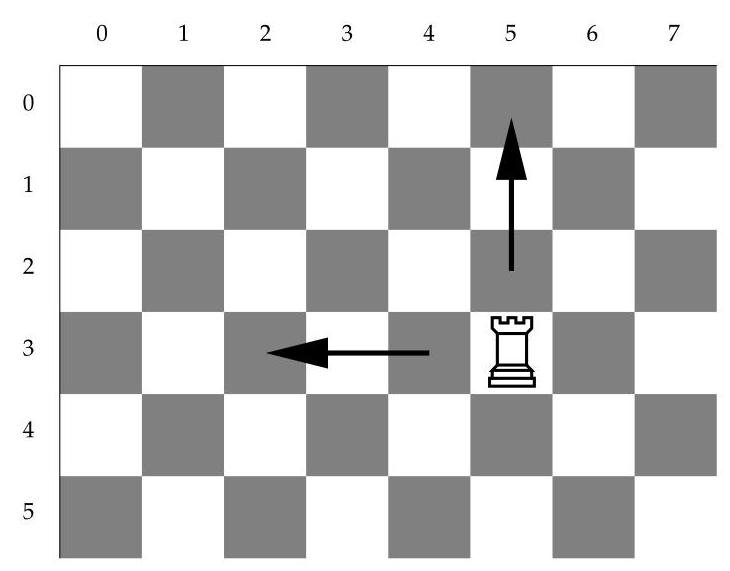
\includegraphics[width=0.72\textwidth]{images/fig-1-1-rook-move.jpg}
\caption{战车移动游戏，玩家可以在国际象棋棋盘上沿箭头方向移动战车。}
\label{fig:1.1}
\end{figure}

图~\ref{fig:1.2}给出了棋盘各局面的尼姆值。左上角方格等价于 $0$，因为战车无法再移动。它下方的方格只能走到值为 $0$ 的方格，所以等价于 \(*1\)，因为 \(\operatorname{mex}\left({\{0\}}\right)=1\)。再往下的方格等价于 \(*2\)，因为它的选项等价于 \(0\) 和 \(*1\)。在最左列中，战车只能向上移动，所以第 \(i\) 行第 0 列的方格显然对应于尼姆堆 \(*i\)。类似地，最上方第 0 行第 \(j\) 列的条目为 \(*j\)。



一般地，若已知某个方格左侧和上方所有方格的尼姆值，也就是该局面的所有选项，就能求出该方格的尼姆值。例如第 3 行第 2 列的方格，其左侧有 \(*3\) 和 \(*2\)，上方有 \(*2,*3,0\)。因此该方格等价于 \(*1\)，因为 \(\operatorname{mex}\left({\{0,2,3\}}\right)=1\)。图~\ref{fig:1.1}中战车所在的第 3 行第 5 列方格，对应条目为 \(*6\)。



\begin{figure}[htbp]
\centering
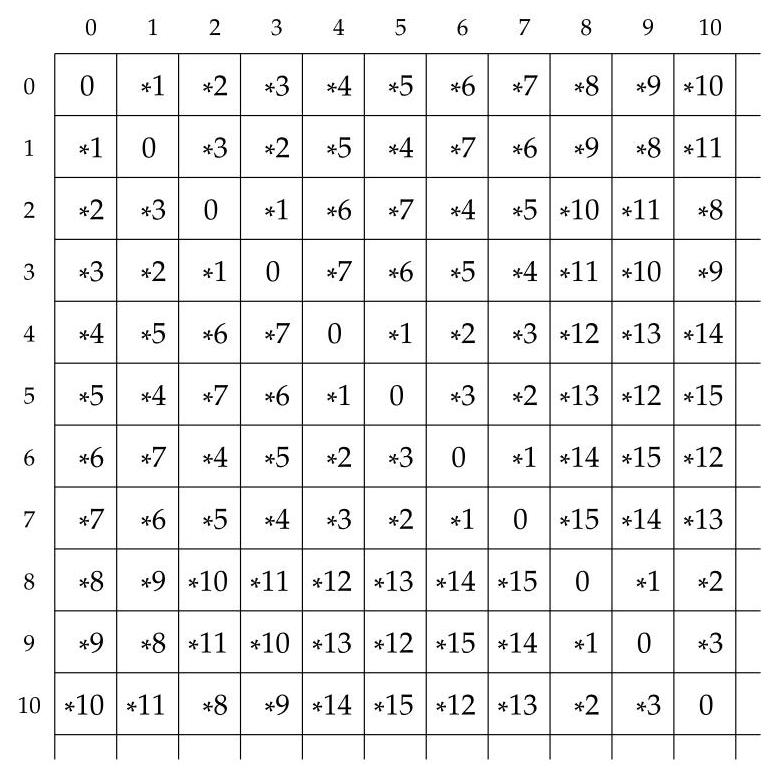
\includegraphics[width=0.78\textwidth]{images/fig-1-2-rook-nim-values.jpg}
\caption{战车移动游戏局势的等价尼姆堆 \(*n\)。}
\label{fig:1.2}
\end{figure}

图~\ref{fig:1.2}显示，棋盘上唯一的必败方格位于主对角线上，它们都等价于 0。直接看也很清楚：左上角方格当然是必败位置；而一旦战车在对角线上，下一步必然离开对角线，对手随后总能把战车移回对角线。

敏锐的读者会注意到，战车移动游戏其实就是两堆尼姆游戏。战车位于第 \(i\) 行第 \(j\) 列时，向上移动就是减小 \(i\)，向左移动就是减小 \(j\)。因此该局面就是 \(*i+*j\)。当且仅当 \(i=j\)，也就是战车在对角线上时，它是必败位置。

尼姆值的作用不止在于区分必胜和必败。当棋盘上放置多个战车时，它尤其有用。若允许多个战车占据同一方格，这就对应于多个战车移动游戏的博弈之和。例如，一个战车在第 2 行第 0 列，另一个在第 4 行第 6 列；这两个战车构成必败位置并不直观，但两个方格的尼姆值都等于 2。

定理~\ref{theo:1.14}指出，任何无偏博弈都等价于某个单一尼姆堆。特别地，两个尼姆堆的和也等价于一个单一尼姆堆。如果暂时忘掉\eqref{eq:1.3}中用二进制求解尼姆游戏的方法，那么到目前为止，我们只知道两个尼姆堆大小不同则必胜、大小相同则必败。图~\ref{fig:1.2}实际上给出了 \(*i+*j\) 的尼姆值计算。

这些尼姆值呈现出明显规律。首先，沿主对角线反射后表格保持对称，因为行和列可以互换。其次，在同一行(或同一列)中，各项互不相同；这是因为对任何整数集合 \(S\)，\(\operatorname{mex}(S)\) 不属于 \(S\)，所以某格的值不可能等于它左侧已有的值。现在取一个 2 的幂，例如 \({2}^{k}\)，并观察编号为 \(0,1,\ldots,{2}^{k}-1\) 的前 \({2}^{k}\) 行和列。表格左上角的这个方块(例如 \(k=2\) 时是 \(4\times4\) 方块)中，每一行、每一列都只出现 \(0,1,\ldots,{2}^{k}-1\) 的某种排列。下一节将精确说明 2 的幂在计算两个尼姆堆之和时的作用，并解释为什么\eqref{eq:1.3}中的二进制表示会自然出现。

\section{尼姆堆之和}

本节推导如何计算一般尼姆局面，也就是若干尼姆堆之和的尼姆值。结果正是前面用二进制表示定义的尼姆和；现在我们用博弈之和与博弈等价的语言重新得到它，而不预先假定二进制算法。

例如，我们已经知道 \(*1+*2+*3\equiv 0\)，所以由引理~\ref{lem:1.12}，\(*1+*2\) 等价于 \(*3\)。不过，一般不能把尼姆堆大小直接做普通加法；因为 \(*2+*3\) 等价于 \(*1\)，而 \(*1+*3\) 等价于 \(*2\)。

若 \(*k\equiv *n+*m\)，就称 \(k\) 为 \(n\) 与 \(m\) 的尼姆和，记作 \(k=n\oplus m\)。下面的定理表明，不同 2 的幂做尼姆和时，结果就是它们的普通算术和。例如 \(1=2^{0}\)、\(2=2^{1}\)，所以 \(1\oplus2=1+2=3\)。

\begin{theorem}\label{theo:1.15}设 \(n \geq  1\) ，且 \(n = {2}^{a} + {2}^{b} + {2}^{c} + \cdots\) ，其中 \(a > b > c > \cdots  \geq  0\) 。那么
\begin{equation}
* n \equiv   * \left( {2}^{a}\right)  +  * \left( {2}^{b}\right)  +  * \left( {2}^{c}\right)  + \cdots .\label{eq:1.19}
\end{equation}
\end{theorem}
先解释这个定理的含义，再给出证明。表达式 \(n={2}^{a}+{2}^{b}+{2}^{c}+\cdots\) 是把 \(n\) 写成若干个不同 2 的幂之和。每个 \(n\) 都有唯一这样的表示。这等价于 \(n\) 的二进制表示：若 \(n<{2}^{a+1}\)，就把 \(n\) 写成 \({2}^{a},{2}^{a-1},{2}^{a-2},\ldots,{2}^{0}\) 的线性组合，每个 2 的幂前面的系数只能是 0 或 1，也就是对应位置的二进制数字。例如，

\[
9 = 8 + 1 = 1 \cdot  {2}^{3} + 0 \cdot  {2}^{2} + 0 \cdot  {2}^{1} + 1 \cdot  {2}^{0},
\]

因此十进制 9 的二进制表示是 1001。定理~\ref{theo:1.15}只保留二进制表示中数字 1 所对应的那些 2 的幂，即 \({2}^{a},{2}^{b},{2}^{c},\ldots\)。

\eqref{eq:1.19}右侧是一个博弈之和。它说明，单个尼姆堆 \(*n\) 等价于若干堆的和，而这些堆的大小正是 \(n\) 的二进制展开中出现的不同 2 的幂。如果像\eqref{eq:1.4}那样用点来表示代币，一个例子是

\[
*14 = ::::::::: \quad\equiv\quad  :::::  +  :: + : 
\]

这里 \(n=14\)。若再有一个尼姆堆 \(*m\)，也把它分解为大小为 2 的幂的若干尼姆堆之和，那么 \(*n+*m\) 就由许多这样的堆组成。相等的堆会成对抵消，因为两个相同博弈的和是必败的，可以忽略。剩下的堆大小互不相同，仍是 2 的幂；把它们相加，就得到与 \(*n+*m\) 等价的单个尼姆堆 \(*k\)。例如，若 \(n=9=8+1\)，且 \(m=14=8+4+2\)，则
\(*n+*m\equiv *8+*1+*8+*4+*2\equiv *4+*2+*1\equiv *7\)，也就是 \(9\oplus14=7\)。特别地，\(*9+*14+*7\) 是必败位置；若没有这个定理，直接证明会相当繁琐。

定理\ref{theo:1.15}的一个推论是，两个整数的尼姆和永远不会超过它们的算术和。此外，如果两个整数都小于某个 2 的幂，那么它们的尼姆和也小于该 2 的幂。

\begin{lemma}\label{lem:1.16}假设定理\ref{theo:1.15} 对于任何满足 \(n < {2}^{d}\) 的 \(n\) 都成立。设 \(0 \leq  p,q < {2}^{d}\) 。那么 \(* p +  * q \equiv   * r\) 其中 \(0 \leq  r < {2}^{d}\) ，即 \(r = p \oplus  q < {2}^{d}\) 。
\end{lemma}

\begin{proof} \(p\) 和 \(q\) 都是小于 \({2}^{d}\) 的不同 2 的幂的和。根据定理 \ref{theo:1.15}， \(r\) 也是这样的 2 的幂的和，其中那些同时出现在 \(p\) 和 \(q\) 中的幂，比如 \({2}^{k}\) ，在博弈之和中会抵消，因为 \(* \left( {2}^{k}\right)  +  * \left( {2}^{k}\right)  \equiv  0\) 。因此，得到的和 \(r\) 也小于 \({2}^{d}\) 。
\end{proof}

通过结合一个例子，比如 \(n = 7\) ，来考虑下面的证明可能会更容易理解。

\begin{proof}[定理 \ref{theo:1.15} 的证明]我们采用归纳法进行证明。考虑某个 \(n\) ，并假设该定理对所有更小的 \(n\) 都成立。设 \(n = {2}^{a} + q\) ，其中 \(q = {2}^{b} + {2}^{c} + \cdots\) 。如果 \(q = 0\) ，该命题显然成立( \(n\) 只是 2 的单一幂次)，所以设 \(q > 0\) 。我们有 \(q < {2}^{a}\) 。根据归纳假设， \(* q \equiv   * \left( {2}^{b}\right)  +  * \left( {2}^{c}\right)  + \cdots\) ，所以为了证明 \eqref{eq:1.19}，我们只需证明 \(* n \equiv   * \left( {2}^{a}\right)  +  * q\) 。我们使用引理~\ref{lem:1.13} 来证明这一点，即通过证明 \(* n\) 的每个选项都等同于博弈 \(* \left( {2}^{a}\right)  +  * q\) 的某个选项，反之亦然。 \(* n\) 的选项是 \(0, * 1, * 2,\ldots , * \left( {n - 1}\right)\) 。

\(* \left( {2}^{a}\right)  +  * q\) 的选项有两种类型，取决于玩家是在尼姆堆 \(* \left( {2}^{a}\right)\) 还是 \(* q\) 中移动。第一种类型的选项由以下给出
 

 

\begin{equation}
\begin{aligned}
    0 + *q &\equiv *r_0 \\
    *1 + *q &\equiv *r_1 \\
    &\vdots \\
    *(2^a - 1) + *q &\equiv *r_{2^a-1}
\end{aligned}
\label{eq:1.20}
\end{equation}



其中，对于 \(0 \leq  i < {2}^{a}\) ， \(* i +  * q\) 与某个尼姆堆\(* {r}_{i}\) 的等价性，即使我们不知道 mex 规则，根据归纳假设也成立。此外，根据引理 \ref{lem:1.16}(对于 \(d = a\) ，因为对于 \(n < {2}^{a}\) ，定理 \ref{theo:1.15} 根据归纳假设成立)， \(i\) 和 \(q\) 都小于 \({2}^{a}\) ，因此 \({r}_{i} < {2}^{a}\) 也小于 \({2}^{a}\) 。在 \eqref{eq:1.20} 的右侧，对于 \(0 \leq  i < {2}^{a}\) 有 \({2}^{a}\) 个尼姆堆 \(* {r}_{i}\) 。我们声称它们都是不同的，所以这些选项恰好构成集合 \(\{ 0, * 1, * 2,\ldots\) ， \(\left. {*\left( {{2}^{a} - 1}\right) }\right\}\) 。即，通过将博弈 \(* q\) 添加到堆 \(* {r}_{i}\) 中，\eqref{eq:1.16} 意味着 \(* {r}_{i} +  * q \equiv\)  \(* i +  * q +  * q \equiv   * i\) ，所以 \(* {r}_{i} \equiv   * {r}_{j}\) 意味着 \(* {r}_{i} +  * q \equiv   * {r}_{j} +  * q\) ，即 \(* i \equiv   * j\) ，因此根据引理~\ref{lem:1.7}，对于 \(0 \leq  i,j < {2}^{a}\) 有 \(i = j\) 。

\(* \left( {2}^{a}\right)  +  * q\) 的第二种类型的选项形式为

\[
* \left( {2}^{a}\right)  + 0 \equiv   * \left( {{2}^{a} + 0}\right)
\]

\[
* \left( {2}^{a}\right)  +  * 1 \equiv   * \left( {{2}^{a} + 1}\right)
\]

\[
\vdots
\]

\[
* \left( {2}^{a}\right)  +  * \left( {q - 1}\right)  \equiv   * \left( {{2}^{a} + q - 1}\right) ,
\]

其中右侧的堆大小再次由归纳假设给出。 这些堆构成集合 \(\left\{  {*\left( {2}^{a}\right) , * \left( {{2}^{a} + 1}\right) ,\ldots , * \left( {n - 1}\right) }\right\}\)。与第一种类型的选项一起，它们恰好是 \(* n\) 的选项。这表明 \(* n\) 的选项和博弈之和 \(* \left( {2}^{a}\right)  +  * q\) 的选项确实是等价的，从而完成了证明。
\end{proof}

在定理\ref{theo:1.15}的证明中，如果 \(n = 7\) ，那么 \(n = {2}^{a} + q\) ，其中 \(a = 2\) 且 \(q = 3\) 。那么\eqref{eq:1.20}中的尼姆堆 \(* {r}_{0}, * {r}_{1}, * {r}_{2}, * {r}_{3}\) 是图~\ref{fig:1.2}中战车移动表第 \(q = 3\) 列前 \({2}^{a}\) 行0、1、2、3中的元素。

定理\ref{theo:1.15}证明中的这一步基于引理\ref{lem:1.16}，它在一定程度上也解释了为什么2的幂次会出现在尼姆和的计算中。在\eqref{eq:1.20}中从 \(* \left( {2}^{a}\right)  +  * q\) 移动的选项恰好能产生数字 \(0,1,\ldots ,{2}^{a} - 1\) ，如果用其他东西代替 \({2}^{a}\) ，这就行不通了。

任何一组数字的尼姆和可以通过将每个数字写成不同2的幂次之和，然后成对消去重复项来得到。对于\eqref{eq:1.3}和\eqref{eq:1.4}中的例子，我们有

\begin{equation}\label{eq:1.21}
4 \oplus  5 \oplus  9 \oplus  {14} = 4 \oplus  \left( {4 + 1}\right)  \oplus  \left( {8 + 1}\right)  \oplus  \left( {8 + 4 + 2}\right)  = 4 + 2 = 6. 
\end{equation}

因此，尼姆局面$(4,5,9,14)$等价于一个大小为 6 的单堆。之所以成立，是因为把这个大小为 6 的堆再加到原来的四堆之和上，会得到必败位置:

\[
\left( {*4 +  * 5 +  * 9 +  * {14}}\right)  +  * 6 \equiv  0.
\]

从\eqref{eq:1.3}中的左表也可以看出这一点。也就是说，尼姆和相当于将堆的大小写成二进制形式，并在每一列(2的幂次)中分别对二进制数字进行模2加法。如果相应的2的幂次出现偶数次(所有对都消去)，尼姆和的列元素为0；如果出现奇数次，则为1。

\section{计算尼姆值}\label{sec-1.8}

在本节中，我们使用定理~\ref{theo:1.14}中的MEX规则来分析一些无偏博弈。

与战车移动游戏类似，图~\ref{fig:1.3}给出了皇后移动博弈：把战车换成国际象棋中的皇后，皇后可以水平、垂直或沿对角线向左、向上移动。因此主对角线上的方格不再必败。这个博弈也可以用两堆代币来描述：一步行动可以像尼姆游戏那样从一堆中取走代币，也可以从两堆中取走相同数量的代币(所以它不再是两个普通尼姆堆的和)。为了说明我们关心的不只是胜负方格，图中还加上了一个大小为 4 的尼姆堆。

\begin{figure}[htbp]
\centering
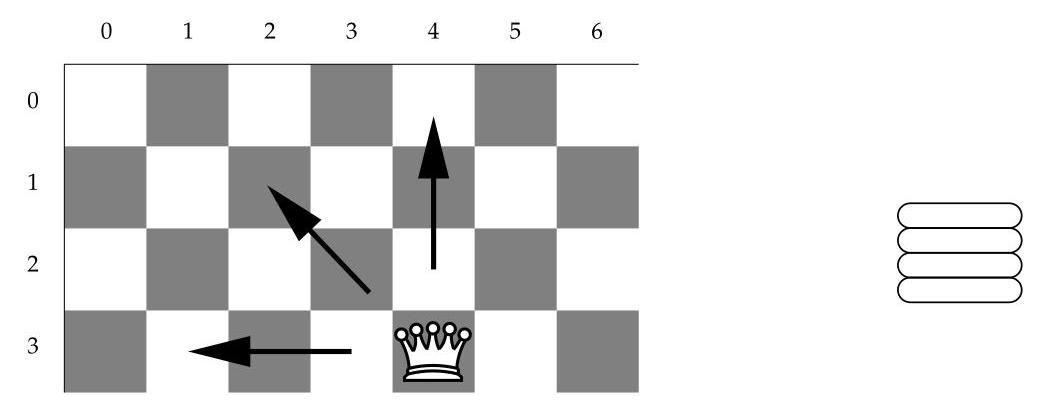
\includegraphics[width=0.76\textwidth]{images/fig-1-3-queen-nim-sum.jpg}
\caption{皇后移动博弈和一个大小为4的尼姆堆的博弈之和。玩家可以要么沿箭头方向移动皇后，要么从堆中取走四个代币中的一些。}
\label{fig:1.3}
\end{figure}

图~\ref{fig:1.4}给出了由 MEX 规则确定的皇后移动博弈各局面的等价尼姆堆。图~\ref{fig:1.3}中，皇后所在的第 3 行第 4 列方格值为 \(*2\)。因此，一个制胜行动是从额外的尼姆堆中取走两枚代币，使它也变成 \(*2\)，从而形成必败局面 \(*2+*2\)。由于 2 是皇后各选项尼姆值的 mex，这些选项中可能包含更高的尼姆值，正如扑克尼姆游戏中那样。事实上，皇后可以走到两个等价于 \(*4\) 的局面，即第 3 行第 1 列和第 0 行第 4 列。如果皇后走到其中之一，就形成 \(*4+*4\)，同样是必败位置；因此这也是图~\ref{fig:1.3}中的另外两种制胜行动。



\begin{figure}[htbp]
\centering
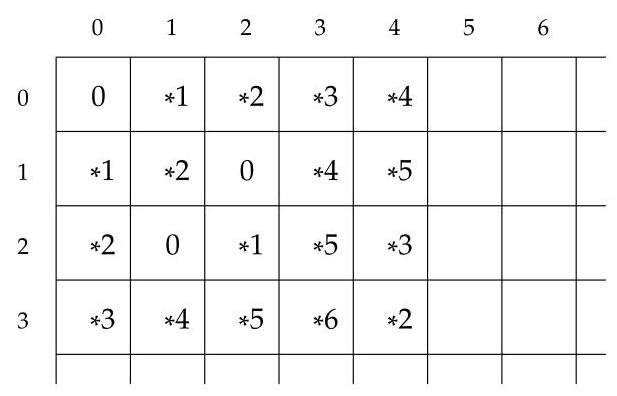
\includegraphics[width=0.62\textwidth]{images/fig-1-4-queen-equivalent-nim.jpg}
\caption{皇后移动博弈局势的等价尼姆堆。}
\label{fig:1.4}
\end{figure}

无偏博弈凯尔斯博弈的玩法如下:给定一排 \(n\) 个保龄球瓶(编号为 \(1,2,\ldots ,n\) )，一次移动可以击倒一个或两个连续的球瓶，就像这个有5个球瓶的例子，其中第2和第3个球瓶被击倒:
\begin{equation}
\label{eq:1.22}
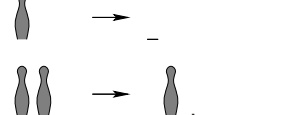
\includegraphics[width=0.42\textwidth]{images/eq-1-22-kayles-move.jpg}
\end{equation}



如果这个博弈被称为 \({K}_{n}\) ，那么击倒单个球瓶 \(p\) 会形成博弈之和 \({K}_{p - 1} + {K}_{n - p}\) ，而击倒球瓶 \(p\) 和 \(p + 1\) (在图中是 \(p = 2\) 和 \(n = 5\) )会形成博弈之和 \({K}_{p - 1} + {K}_{n - p - 1}\) (这里是 \({K}_{1} + {K}_{2}\) )。 \({K}_{n}\) 的选项是所有可能的 \(p\) 对应的这些博弈之和，由于球瓶行的对称性， \(p\) 只需要考虑到中间的球瓶即可。注意，在这个博弈中，选项恰好是博弈的和。对于 mex 规则，只有它们的尼姆值是重要的。下图展示了有 1、2 或 3 个球瓶的凯尔斯博弈的所有选项:

\begin{center}
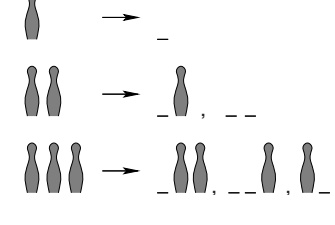
\includegraphics[width=0.45\textwidth]{images/inline-1-kayles-options-1-3.jpg}
\end{center}


这表明 \({K}_{1} \equiv   * \operatorname{mex}\left( 0\right)  =  * 1,{K}_{2} \equiv   * \operatorname{mex}\left( {1,0}\right)  =  * 2\) ，并且 \({K}_{3} \equiv   * \operatorname{mex}\left( {2,1,1 \oplus  1}\right)  =\)  \(* 3\) ，因为 \(1 \oplus  1 = 0\) 。有 4 个球瓶的凯尔斯博弈的选项是

\begin{center}
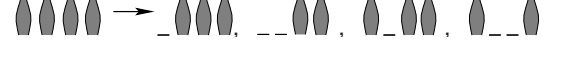
\includegraphics[width=0.72\textwidth]{images/inline-1-kayles-options-4.jpg}
\end{center}


因此 \({K}_{4} \equiv   * \operatorname{mex}\left( {3,2,1 \oplus  2,1 \oplus  1}\right)  =  * \operatorname{mex}\left( {3,2,3,0}\right)  =  * 1\) ，这导致了有 6 个球瓶时一个意想不到的必胜步:

\begin{center}
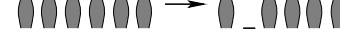
\includegraphics[width=0.45\textwidth]{images/inline-1-kayles-winning-6.jpg}
\end{center}

为了验证这一点，可以直接为 \({K}_{1}+{K}_{4}\) 的每个选项找出一个走向必败位置的回应，从而证明所有选项都是必胜位置，也就证明 \({K}_{1}+{K}_{4}\) 本身必败。这个练习很有启发性。

练习中描述了更多的无偏博弈。

\section{有偏博弈简介} \label{sec-1.9}

如果在一个博弈位置中，两个玩家可用的行动可能不同，那么这个组合博弈就被称为有偏博弈。这些博弈有丰富的理论，我们在这里概述其最初的概念，特别是四种结果类，以及在某些博弈中作为位置强度的数字，这是由康威(2001 年)开创的。

两个玩家分别称为左玩家和右玩家。考虑纵横棋博弈，它由一个方格棋盘给出(起始位置通常是矩形，但不必如此)，在每一步中，左玩家可以用一个垂直的多米诺骨牌占据两个垂直相邻的空格，右玩家可以用一个水平的多米诺骨牌占据两个水平相邻的空格。(至少小写字母“l”比字母“r”更垂直，这样可以记住这一点。)因此，从一个 3 行 2 列的棋盘开始，在考虑对称性的情况下，我们有
\begin{equation}
\label{eq:1.23}
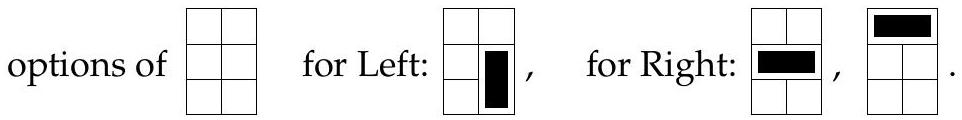
\includegraphics[width=0.82\textwidth]{images/eq-1-23-domineering-options.jpg}
\end{equation}
这个博弈与无偏博弈塞砖棋(见练习~\ref{exer:1.4})非常不同，在塞砖棋中，每个玩家可以以任意方向放置多米诺骨牌。如\eqref{eq:1.23}所示，在纵横棋中，左玩家和右玩家的选项通常是不同的。和之前一样，我们假设采用正常规则，即无法再行动的玩家输。



我们总是假设玩家采取最优策略。在\eqref{eq:1.23}中，这意味着右玩家会选择第一个选项，将多米诺骨牌放在中间，之后左玩家就无法再行动了，而第二个选项留下一个 \(2 \times  2\) 棋盘会给左玩家提供两步额外的行动。

如引理~\ref{lem:1.1} 所述，无偏博弈只有失败或必胜两种情况。对于有偏博弈，有四种可能的结果类，用以下花体字母表示:

\(\mathcal{L}\) :无论谁先行动，左玩家必胜。

\(\mathcal{R}\) :无论谁先行动，右玩家必胜。

\(\mathcal{P}\) :先行动的玩家失败，因此前一个玩家获胜。

\(\mathcal{N}\) :先行动的玩家获胜。(有时称为“下一玩家”，尽管这和“下周五”一样模棱两可，因为实际上是当前玩家获胜。)

每个博弈都恰好属于这些结果类之一。\(\mathcal{P}\) 局面就是前面说的必败位置，\(\mathcal{N}\) 局面就是必胜位置。对有偏博弈(partizan game)来说，还必须考虑另外两类 \(\mathcal{L}\) 和 \(\mathcal{R}\)。在纵横棋(Domineering)中，一个至少含两个方格的竖条，最小形式为 -，属于 \(\mathcal{L}\) 类；相应的横条属于 \(\mathcal{R}\) 类。\eqref{eq:1.23}中的起始 \(3\times2\) 棋盘属于 \(\mathcal{N}\) 类。

在\eqref{eq:1.23}中，Right 的第一步创造出两个互不相连的 \(1\times2\) 博弈；和前面一样，这表示一个博弈之和(game sum)。若对任意其他博弈 \(J\)，\(G+J\) 与 \(H+J\) 总属于同一结果类，则称 \(G\) 与 \(H\) 等价，记为 \(G\equiv H\)。这扩展了定义~\ref{def:1.5}。每个必败博弈(\(\mathcal{P}\) 类中的任意博弈)都等价于没有选项的零博弈 0，论证与引理~\ref{lem:1.8}相同。因此，引理~\ref{lem:1.10}仍然成立：加上一个必败博弈不会改变原博弈的结果类。

对于任何有偏博弈 \(G\) ，存在一个负博弈 \(- G\) ，使得如 \eqref{eq:1.13} 中所述的 \(G + \left( {-G}\right)  \equiv  0\) 成立。这个负博弈是通过交换 Left 和 Right 的选项，并对它们的选项进行递归交换得到的。对于纵横棋(Domineering)，任何博弈位置 \(G\) 的负博弈(由尚未被多米诺骨牌(domino)占据的方格表示)是通过将棋盘旋转 90 度得到的。例如，
\begin{equation}
\label{eq:1.24}
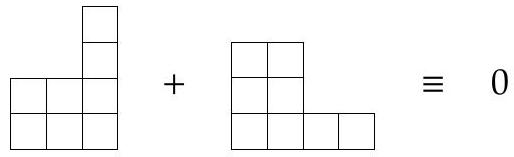
\includegraphics[width=0.55\textwidth]{images/eq-1-24-domineering-negative.jpg}
\end{equation}
因为一个组件中玩家的任何行动都可以被另一个玩家在另一个组件中进行相应的行动所复制。通过这种方式，第二个玩家总是有行动可做，并且当达到 \(0 + 0\) 局势时获胜。

形式上，一个博弈 \(G\) 由两组博弈 \({\mathcal{G}}^{L}\) 和 \({\mathcal{G}}^{R}\) 定义，它们分别定义了 Left 和 Right 的选项。那么 \(G\) 可以写成 \(\left\{  {{\mathcal{G}}^{L} \mid  {\mathcal{G}}^{R}}\right\}\) 。在具体例子中，人们直接列出集合 \({\mathcal{G}}^{L}\) 和 \({\mathcal{G}}^{R}\) 的元素，而不是使用集合符号。例如，如果 \({\mathcal{G}}^{L} = {\mathcal{G}}^{R} = \varnothing\) ，那么我们将这个博弈写成 \(\{ \left| {\} \text{ rather than }\{ \varnothing }\right| \varnothing \}\) 。这是可能的最简单的博弈，任何玩家都没有选项，我们用 0 来表示:

\begin{equation}
\label{eq:1.25}
0 = \{  \mid  \} \text{ . }
\end{equation}

博弈中的选项是递归定义的。我们可以将 \eqref{eq:1.23} 写成
\begin{equation}
\label{eq:1.26}
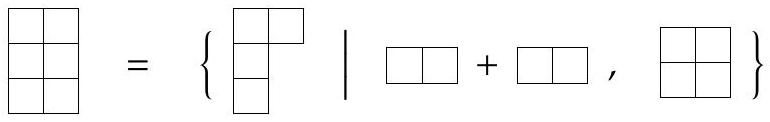
\includegraphics[width=0.70\textwidth]{images/eq-1-26-domineering-recursive.jpg}
\end{equation}


并继续定义
\begin{equation}
\label{eq:1.27}
\square = \{0,\square \mid \square\},
\end{equation}

其中 Left 的第一个选项是将多米诺骨牌(domino)放在左上角，这使得 Right 没有进一步的行动，第二个(较差的)选项是将多米诺骨牌放在底部；Right 只有一种选择。此外，

\begin{equation}
\label{eq:1.28}
\square  = \left\{  {0|}\right\}  ,\;\square \square  = \left\{  {0|0}\right\}  ,
\end{equation}

这些是 Left 或 Right 分别只剩下一步行动，而另一个玩家没有行动的局势。\eqref{eq:1.26} 中 Right 的第一个选项也可以通过博弈之和的递归定义来定义为

\[
\square \square  + \square \square  = \left\{  {\square \square }\right\}  ,
\]

\eqref{eq:1.26} 中 Right 的第二个选项定义为
\begin{equation}
\label{eq:1.29}
\square = \{\square \mid \square\}.
\end{equation}
定义 \eqref{eq:1.25} 到 \eqref{eq:1.29} 通过引用更简单的博弈进行递归定义，所示的棋盘配置作为合适的占位符。重要的是在后续的最优玩法中哪个玩家最终失败。

在\eqref{eq:1.27}中，Left 有一个被占优选项[1]，理性玩家永远不应选择它，因为这样会白白让 Right 多走一步。被占优选项可以省略，从而简化博弈的递归描述。

注意:在无偏博弈塞砖棋(Cram)的棋盘布局1中，没有被占优选项。

在塞砖棋(Cram)中，这种布局等价于大小为 2 的尼姆堆 \(*2\)。它有两个选项 \(*1\) 和 0，且二者互不占优。例如，在博弈之和 \(*2+*1\) 中，走到 \(*1+*1\) 是制胜行动，这就需要用到 \(*2\) 的选项 \(*1\)。无偏博弈(impartial game)恰好是满足 \(\left\{ {{\mathcal{G}}^{L}\mid{\mathcal{G}}^{R}}\right\}\) 且 \({\mathcal{G}}^{L}={\mathcal{G}}^{R}\) 的博弈，并且其选项本身也都是无偏博弈。由\eqref{eq:1.25}可知，最简单的无偏博弈是 0；次简单的是 \(\{0\mid0\}\)，也就是大小为 1 的尼姆堆 \(*1\)，通常也写作 \(*\)。

在有偏博弈(partizan game)中，一个重要的新概念是“数”。它适用于某些有偏博弈，但不是全部。如果一个博弈可以表示为一个数，这个数就表示 Left 在该博弈中安全领先的步数。最简单的数是整数，但也可以出现某些分数。例如，纵横棋(Domineering)中的竖条局面可以表示为整数 1。并且 \(1+1=2\)，也就是说，数的博弈之和对应于普通算术加法。类似地，纵横棋中对应于 \(-1\) 的横条局面满足 \(1+\left({-1}\right)\equiv0\)。对于正整数 \(n\)，若 Left 领先 \(n\) 步并走掉其中一步，之后仍领先 \(n-1\) 步。于是可用 \(n\) 表示该博弈，并得到递归定义

\begin{equation}
\label{eq:1.30}
n = \{ n - 1 \mid  \} ,
\end{equation}

它的基础情况是 \(1 = \{ 0 \mid  \}\) ，如\eqref{eq:1.28}所示。负整数对应的博弈被定义为正整数对应博弈的负博弈(negative game) \(- n\) 。在博弈 \(- n\) 中，后手玩家(右方)领先 \(n\) 步。

注意：除 0 之外，没有无偏博弈可以表示为数。\eqref{eq:1.18}中定义的尼姆堆完全不同，它遵循的是 \(*n+*n\equiv0\) 这样的规则。尼姆堆有时称为“尼姆数”(nimber)，以区别于普通的数。

为了更一般地定义数，我们需要在博弈上定义一个偏序(partial order) \(\geq\) (它不是“比……更简单”的顺序)，定义如下:

\begin{equation}
\label{eq:1.31}
\begin{aligned}
G \geq H \Leftrightarrow {}&
(\forall J : H + J \in \mathcal{L} \cup \mathcal{N} \Rightarrow G + J \in \mathcal{L} \cup \mathcal{N},\\
&\forall J : H + J \in \mathcal{L} \cup \mathcal{P} \Rightarrow G + J \in \mathcal{L} \cup \mathcal{P}).
\end{aligned}
\end{equation}

其中，如果先手玩家(左方)先走能获胜，则一个博弈属于 \(\mathcal{L} \cup  \mathcal{N}\) ；如果先手玩家(左方)后走能获胜，则属于 \(\mathcal{L} \cup  \mathcal{P}\) 。有了这个理解，\eqref{eq:1.31}可以写成

\[
G \geq  H \Leftrightarrow  \left( {\forall J : \text{ Left wins in }H + J \Rightarrow  \text{ Left wins in }G + J}\right) .
\]

也就是说，如果无论在什么情况下(始终假设是最优玩法)，用 \(G\) 替换 \(H\) 都不会对先手玩家(左方)造成不利，那么就有 \(G \geq  H\) 。那么 \(\geq\) 是博弈上的一个偏序，因为它显然是自反的(reflexive)和传递的(transitive)，并且在博弈等价的意义下是反对称的(antisymmetric):

\begin{lemma}\label{lem:1.17}\(G \geq  H\) 且 \(H \geq  G \Leftrightarrow  G \equiv  H\) 。
\end{lemma}
\begin{proof}回想一下， \(G \equiv  H\) 意味着对于任何博弈 \(J\) ， \(G + J\) 和 \(H + J\) 属于同一个结果类 \(\mathcal{L},\mathcal{R},\mathcal{P},\mathcal{N}\) ，所以 “ \(\Leftarrow\) ” 是显然的。为了证明 “ \(\Rightarrow\) ”，假设 \(G \geq  H\) 且 \(H \geq  G\) ，并设 \(J\) 为任意博弈。如果 \(H + J \in  \mathcal{L}\) ，那么由 \eqref{eq:1.31} 可得 \(G + J \in  \left( {\mathcal{L} \cup  \mathcal{N}}\right)  \cap  \left( {\mathcal{L} \cup  \mathcal{P}}\right)  = \mathcal{L}\) ，因为结果类是不相交的。由对称性可知，如果 \(G + J \in  \mathcal{L}\) ，那么 \(H + J \in  \mathcal{L}\) 。接下来，考虑结果类 \(\mathcal{P}\) :如果 \(H + J \in  \mathcal{P}\) ，那么由 \eqref{eq:1.31} 可得 \(G + J \in  \mathcal{L} \cup  \mathcal{P}\) 。如果 \(G + J \in  \mathcal{L}\) ，那么正如刚才所证 \(H + J \in  \mathcal{L}\) ，但 \(H + J \in  \mathcal{P}\) 与 \(\mathcal{L}\) 不相交，所以 \(G + J \in  \mathcal{P}\) 。由对称性可知，如果 \(G + J \in  \mathcal{P}\) ，那么 \(H + J \in  \mathcal{P}\) 。类似的论证适用于结果类 \(\mathcal{R}\) 和 \(\mathcal{N}\) 。
\end{proof}


将 \(G < H\) 定义为 \(H \geq  G\) 且非 \(G \equiv  H\) 。这允许对作为数字的有偏博弈进行如下递归的定义。

\begin{definition}\label{def:1.18}一个博弈 \(G = \left\{  {{\mathcal{G}}^{L} \mid  {\mathcal{G}}^{R}}\right\}\) 是一个数字，如果 \(G\) 的所有左选项 \({G}^{L} \in  {\mathcal{G}}^{L}\) 和 \(G\) 的所有右选项 \({G}^{R} \in  {\mathcal{G}}^{R}\) 都是数字，并且满足 \({G}^{L} < G < {G}^{R}\)。
\end{definition}
最简单的数字是 \(0 = \{  \mid  \}\) ，因为它没有左选项或右选项，所以对于 \(G = 0\) 的条件 \({G}^{L} < G < {G}^{R}\) 显然成立。类似地，对于正整数 \(n\) 在 \eqref{eq:1.30} 中定义的博弈是一个数字，因为它的左选项满足 \(n - 1 < n\) ，并且它没有右选项。

定义 \ref{def:1.18} 中不等式 \({G}^{L} < G < {G}^{R}\) 的直观理解是，在一个数字博弈中移动时，玩家放弃了安全优势，从而削弱了自己的局面，因此移动到左选项 \({G}^{L}\) 会削弱左方( \({G}^{L} < G\) )的局面，而移动到右选项 \({G}^{R}\) 会削弱右方 \(\left( {G < {G}^{R}}\right)\) 的局面。

在一个数字博弈中移动所放弃的优势可能很小，因为博弈也可以是分数形式的数字。例如，纵横棋

\eqref{eq:1.27} 中的局面 1 由 \(\{ 0, - 1 \mid  1\}\) 给出(或者，因为 -1 被占优，由 \(\{ 0 \mid  1\}\) 给出)。

其中 \(0 = \{ \left| \right| \}\) 和 \(1 = \{ 0 \mid  \}\) 根据 \eqref{eq:1.30}，因此根据定义~\ref{def:1.18} 它是一个数。那个数是分数 \(\frac{1}{2}\) ，也就是说，在这个博弈中先手玩家(左玩家)领先半手，因为 \(\frac{1}{2} + \frac{1}{2} + \left( {-1}\right)  \equiv  0\) ，即\eqref{eq:1.32}


\begin{equation}
\label{eq:1.32}
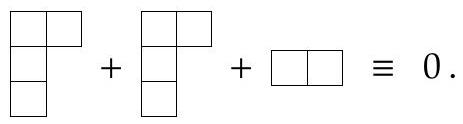
\includegraphics[width=0.55\textwidth]{images/eq-1-32-domineering-half.jpg}
\end{equation}

这可以从(本质上唯一的)最优走法序列推断出来

\begin{center}
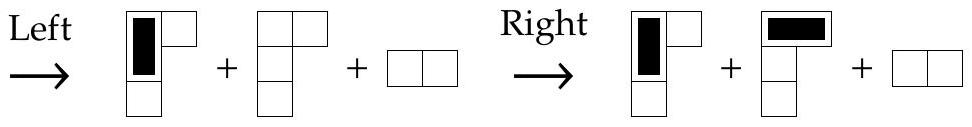
\includegraphics[width=0.55\textwidth]{images/inline-1-eq-1-32-left-starts.jpg}
\end{center}

\begin{center}
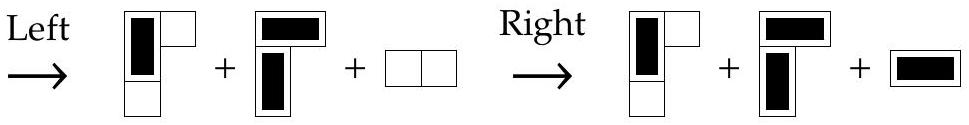
\includegraphics[width=0.55\textwidth]{images/inline-1-eq-1-32-right-starts.jpg}
\end{center}

这表明左玩家作为起始玩家会失败，同样，右玩家作为起始玩家也会失败。

就递归定义的博弈而言，从 \(0 = \{  \mid  \}\) 的定义开始，\eqref{eq:1.32} 表明

\begin{equation}
\label{eq:1.33}
\{ 0 \mid  1\}  + \{ 0 \mid  1\}  + \left( {-1}\right)  \equiv  0. 
\end{equation}

这与 \eqref{eq:1.32} 中纵横棋(Domineering)走法的原因相同，只是更抽象一些。回想一下 \(- 1 = \{  \mid  0\}\) (这对右玩家来说是一步安全走法)。在 \eqref{eq:1.33} 的博弈之和 \(\{ 0 \mid  1\}  + \{ 0 \mid  1\}  + \{  \mid  0\}\) 中，左玩家只能在组件 \(\{ 0 \mid  1\}\) 中走棋，所以下一个博弈状态是 \(0 + \{ 0 \mid  1\}  + \{  \mid  0\}  = \{ 0 \mid  1\}  + \{  \mid  0\}\) 。在这里，右玩家有一个选择，要么在第一个组件中走到 \(1 + \{  \mid  0\}\) ，这是 \(1 + \left( {-1}\right)  = 0\) 且对接下来走棋的左玩家来说是失败局面，要么在第二个组件中(使用他的安全走法)走到 \(\{ 0 \mid  1\}  + 0 = \{ 0 \mid  1\}\) ，这对左玩家来说是胜利局面。显然，右玩家应该选择前者。因此，左玩家作为起始玩家在 \(\{ 0 \mid  1\}  + \{ 0 \mid  1\}  + \{ 0 \mid  1\}\) 中失败。通过非常类似的推理，右玩家作为起始玩家也会失败，这就证明了 \eqref{eq:1.33}。

作为这个论证的扩展，对于每个正整数 \(p\) ，都有一个可以与分数 \(\frac{1}{{2}^{p}}\) 对应的博弈，其递归定义如下:

\begin{equation}
\label{eq:1.34}
\frac{1}{{2}^{p}} = \left\{  {0\left| {\;\frac{1}{{2}^{p - 1}}}\right. }\right\}  \;\text{ and hence }\;\frac{-1}{{2}^{p}} = \left\{  {\left. \frac{-1}{{2}^{p - 1}}\right| \;0}\right\}  . 
\end{equation}

为了证明

\begin{equation}
\label{eq:1.35}
\frac{1}{{2}^{p}} + \frac{1}{{2}^{p}} + \frac{-1}{{2}^{p - 1}} \equiv  0, 
\end{equation}

可以发现，在这个博弈之和中，对于两个玩家来说，在组件 \(\frac{1}{{2}^{p}}\) 中走棋比在 \(\frac{-1}{{2}^{p - 1}}\) 中走棋更好，因为在 \(\frac{-1}{{2}^{p - 1}}\) 中玩家会放弃更多，这与 \eqref{eq:1.33} 的推理类似。因此，无论谁先开始，两步之后局面 \eqref{eq:1.35} 就会变成失败位置 \(\frac{1}{{2}^{p - 1}} + \frac{-1}{{2}^{p - 1}}\) ，这就证明了 \eqref{eq:1.35}。

以下是一个更一般的、递归定义的博弈，其值是分母为 2 的幂的分数。

\begin{definition}\label{def:1.19}设 \(p\) 是一个正整数， \(m\) 是一个奇数。通过以下方式定义博弈 \(\frac{m}{{2}^{p}}\)

\begin{equation}
\label{eq:1.36}
\frac{m}{{2}^{p}} = \left\{  {\left. \frac{m - 1}{{2}^{p}}\right| \;\frac{m + 1}{{2}^{p}}}\right\}  .
\end{equation}
\end{definition}


在 \eqref{eq:1.36} 的右边， \(m - 1\) 和 \(m + 1\) 是偶数，并且我们假设得到的分数像通常那样进行了最大程度的约分，所以它们的分母更小，或者像 \eqref{eq:1.30} 中那样是整数。因此，\eqref{eq:1.36} 是一个递归定义。\eqref{eq:1.36} 的一个例子是 \(\frac{17}{8} = \left\{  {\frac{16}{8}\left| {\;\frac{18}{8}}\right. }\right\}   = \left\{  {2\left| {\;\frac{9}{4}}\right. }\right\}\) 。

方程 \eqref{eq:1.33} 证明了定义 \(\frac{1}{2} = \{ 0 \mid  1\}\) 的合理性。类似地，必须证明 \eqref{eq:1.36} 中的博弈 \(\frac{m}{{2}^{p}}\) 是一个数，并且

\begin{equation}
\label{eq:1.37}
\frac{m}{{2}^{p}} + \frac{m}{{2}^{p}} + \frac{-m}{{2}^{p - 1}} \equiv  0 
\end{equation}

这可以通过使用 \eqref{eq:1.36} 中 \(G = \frac{m}{{2}^{p}}\) 的递归定义来完成，即 \(G = \left\{  {{G}^{L} \mid  {G}^{R}}\right\}\) 且 \({G}^{L} = \frac{m - 1}{{2}^{p - 1}}\) 和 \({G}^{R} = \frac{m + 1}{{2}^{p - 1}}\) 。根据定义~\ref{def:1.18}，我们还必须证明 \({G}^{L} < G\) 和 \(G < {G}^{R}\) 。具体细节请参考 Albert、Nowakowski 和 Wolfe(2007 年)的第 4 章和第 5 章。练习~\ref{exer:1.14} 要求计算一些代表黑白哈肯布什游戏(Black - White Hackenbush)位置的数，作为 \eqref{eq:1.37} 的特殊情况。

根据定义~\ref{def:1.19}，每个分母为 \({2}^{p}\)(其中 \(p\) 为正整数)的有理数都可以表示为一个博弈。在这样的博弈中，行动者每走一步都会放弃 \(\frac{1}{{2}^{p}}\) 步安全优势。在若干数的博弈之和中，玩家会优先在分母最大的分量中行动，因为在那里放弃的优势最少。博弈之和也可能包含非数分量，例如尼姆堆。避数定理指出，玩家应先处理这些非数分量，最后再在数分量中行动。

并非所有有偏博弈(partizan game)都是数。实际上，有些博弈不是数，因为在这些博弈中行动会带来额外的优势。例如，\eqref{eq:1.29} 中的 \(2 \times  2\) 纵横棋(Domineering)棋盘等于 \(\{ 1 \mid   - 1\}\) 。这被称为热情博弈(hot game)，因为在那里行动会以额外步数的形式给玩家带来额外的优势。由 \eqref{eq:1.26} 可知等于 \(\left\{  {\frac{1}{2} \mid   - 2}\right\}\) 的 \(3 \times  2\) 纵横棋棋盘也是热情博弈。相反，数是冷静博弈(cold game)。

如果博弈之和中有几个热情分量，分析它们的热度对于决定先在何处行动很有意义。这已应用于一些具有不相连部分的围棋局面。在国际象棋中，不同的走法很少涉及游戏的不相连部分。然而，国际象棋有相关的发展节奏概念，这可能会超过物质优势。

至此，我们对有偏博弈理论的初步探讨结束。下一节将给出关于该主题的进一步评论以及文献参考。

\section{延伸阅读}

Albert、Nowakowski 和 Wolfe(2007 年)编写的一本关于组合博弈的本科教材，我们采用了其中“自上而下归纳(top - down induction)”这一名称。这本书从许多博弈的例子入手，深入探讨了点格棋(Dots and Boxes)博弈，并处理了短博弈理论，在该理论中(正如我们始终假设的那样)每个位置只有有限个选项，并且不会重复访问任何博弈位置(在“循环”博弈中这是允许的，并且可能导致平局)。一本权威的研究生教材是 Siegel(2013 年)的著作，它在深入处理每个主题之前给出了精彩的概述，包括较新的研究进展。它强调了我们在 1.4 节中讨论的博弈等价概念。

关于组合博弈理论的经典著作是 Berlekamp、Conway 和 Guy(2001 - 2004 年)的《Winning Ways》。其诙谐的语言、生动的彩色插图以及所涉及的大量博弈，使其成为极具吸引力的原始资料。然而，其数学内容较难，并且最好先了解该主题的大致内容；例如，博弈的等价性相当隐晦，被写成了相等。

所有这些书籍都直接讨论有偏博弈。除了在 1.8 节中对有偏博弈的简要介绍外，我们选择专注于较简单的无偏博弈(impartial game)。若要更详细地研究将博弈表示为数的内容，请参阅 Albert、Nowakowski 和 Wolfe(2007 年，第 5.1 节)，其中定义 5.12 就是我们的定义~\ref{def:1.18}。

基于二进制的尼姆必胜策略最早由布顿(Bouton，1901年)提出。皇后移动游戏由维托夫(Wythoff，1907年)提出，他将其描述为尼姆游戏的扩展。每个无偏博弈都等价于某个尼姆堆这一发现，分别归功于斯普拉格(Sprague，1935年)和格鲁迪(Grundy，1939年)。因此，这一理论也称为无偏博弈的斯普拉格-格鲁迪理论(Sprague-Grundy theory)，尼姆值也称为斯普拉格-格鲁迪值或简称格鲁迪值。

1.5 节中对 MEX 规则的处理，受到 Berlekamp、Conway 和 Guy(2001--2004年)著作第 4 章的启发。该章讨论了扑克尼姆、战车和皇后移动游戏、诺斯科特游戏(练习~\ref{exer:1.8})；第 5 章讨论了凯尔斯博弈(Kayles)和拉斯克尼姆游戏(在练习~\ref{exer:1.12}中称为分裂尼姆)。巧取游戏(Chomp，练习~\ref{exer:1.5}和\ref{exer:1.10})由 Gale(1974年)提出；其推广可参考 Gale 和 Neyman(1982年)。练习~\ref{exer:1.9}中的有向图博弈(digraph game)也是理解 mex 规则的好例子，它由 Fraenkel(1996年)提出。

对有偏博弈(partizan game)之和的系统研究使《制胜之道》(Winning Ways)的作者之一约翰·康威(John Conway)认识到，可以用一种优雅的方式将实数(实际上是一种称为超实数的推广)定义为某些博弈中局势的强度。一个数是如定义~\ref{def:1.18}中的博弈 \(G\) ，但左选项 \({G}^{L}\) 的集合 \({\mathcal{G}}^{L}\) 和右选项 \({G}^{R}\) 的集合 \({\mathcal{G}}^{R}\) 可以是无限集。条件 \({G}^{L} < G < {G}^{R}\) 推广了“戴德金分割(Dedekind cut)”，这是实数的一种标准构造方法。原始思想在康威(Conway，2001年)所著的《论数字与博弈》(ONAG，“On Numbers and Games”)中有所描述，这也是一本经典著作。关于入门介绍可参考康威(Conway，1977年)的书。

贝沃斯多夫(Bewersdorff，2005年)对客厅游戏进行了既有知识性又有趣味性的数学研究，并附有详细的历史注释。该书第二部分讨论了组合博弈。

\section{第1章练习}

\begin{exercise}\label{exer:1.1}在做本题时，要注意仅使用定义，而不要依赖你对符号 \(\leq\) 和 \(<\) 的熟悉直觉。考虑一个具有二元关系 \(<\) 的集合 \(S\) ，该关系是传递的，并且对于 \(S\) 中的所有 \(x\) 都满足

\begin{equation}
\label{eq:1.38}
\text{ not }x < x\;\text{ ( } < \text{ is irreflexive). } 
\end{equation}

通过\eqref{eq:1.7}式在 \(S\) 上定义关系 \(\leq\) ，即 \(x \leq  y \Leftrightarrow  x < y\) 或 \(x = y\) 。

(a) 证明 \(\leq\) 是一个偏序(partial order)，并且 \(<\) 可通过\eqref{eq:1.6}式从 \(\leq\) 得到，即 \(x < y \Leftrightarrow  x \leq  y\) 且 \(x \neq  y\) 。

(b) 证明如果 \(<\) 是通过\eqref{eq:1.6}式从一个偏序 \(\leq\) 得到的，那么 \(<\) 是传递且非自反的，并且\eqref{eq:1.7}式成立，即 \(x \leq  y \Leftrightarrow  x < y\) 或 \(x = y\) 。
\end{exercise}

\begin{exercise}\label{exer:1.2}
考虑有若干堆代币的尼姆游戏。玩家轮流从其中一堆中取走一些代币。取走最后一个代币的玩家获胜。在证明(a)部分时，尽量不参考尼姆游戏的最优玩法的二进制表示。

(a) 对所有三堆代币且其中一堆只有一枚代币的局面，准确描述哪些是必败位置。说明你的答案为何正确，可以用归纳法证明，也可以使用尼姆游戏定理。[提示:从简单情况入手寻找规律。]

(b) 考虑三堆代币的尼姆游戏，三堆大小为连续整数，例如$(2,3,4)$。证明唯一的必败局面是$(1,2,3)$，其余情况都是必胜位置。[提示:使用(a)的结论。]

(c) 使用堆大小的二进制表示，找出尼姆局面$(8,11,13)$的所有初始制胜行动。
\end{exercise}
\begin{exercise}\label{exer:1.3}
反向尼姆游戏(misère Nim)的规则与普通尼姆相同，只是最后行动的玩家输。因此，只有一枚代币的单堆就是必败位置(轮到行动的玩家必须取走它)。另一个必败位置是三个各含一枚代币的尼姆堆。

(a) 确定有一堆或两堆时，反向尼姆游戏的必胜位置和必败位置，并给出必胜位置中的制胜行动。

(b) 在反向尼姆游戏中，局面$(1,2,3)$是必胜位置还是必败位置？

(c) 尝试描述任意堆数下反向尼姆游戏的必败位置。[提示:它们与正常规则下尼姆游戏的必败位置密切相关。]
\end{exercise}

\begin{exercise}\label{exer:1.4}
无偏博弈(impartial game)塞砖棋(Cram)在一个 \(m \times  n\) 方格的棋盘上进行，玩家轮流在棋盘上放置一块多米诺骨牌(domino)，该骨牌覆盖两个相邻的空格(尚未被多米诺骨牌占据)，可以是垂直或水平放置。

第一个无法再放置多米诺骨牌的玩家输。 \(2 \times  3\) 棋盘的示例玩法:

\begin{center}
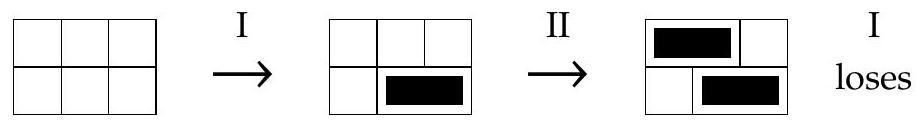
\includegraphics[width=0.65\textwidth]{images/exer-1-4-cram.jpg}
\end{center}

(a) 在 \(3 \times  3\) 塞砖棋中谁会赢？[提示:利用对称性研究可能走法；记住，找到一种必胜策略就足够了。]

(b) 当 \(m\) 和 \(n\) 都是偶数时，在 \(m \times  n\) 的塞砖棋中谁会赢？(该玩家有一个简单且可精确定义的必胜策略，你必须找到它。)

(c) 当 \(m\) 是奇数且 \(n\) 是偶数时，在 \(m \times  n\) 的塞砖棋中谁会赢？(利用(b)的结果很容易得出。)

注意(不是问题)：由于(b)和(c)已经给出答案，这个游戏在 \(m \times n\) 棋盘上实际对局时，通常在 \(m,n\) 都为奇数时更有趣。例如，可以和朋友玩 \(5\times5\) 棋盘。局面常会分解成若干独立部分，比如由 2、3、4、5、6 个方格组成的连续区域；这些区域的胜负已知，可能有助于分析局势。
\end{exercise}

\begin{exercise}\label{exer:1.5}
考虑以下巧取游戏(Chomp):给定一个由 \(m \times  n\) 个点组成的矩形阵列，有 \(m\) 行和 \(n\) 列，就像下一张图左边的 \(3 \times  4\) 那样。位于第 \(i\) 行(从顶部开始)和第 \(j\) 列(从左边开始)的点被命名为(i, j)。一步行动包括选择一个点(i, j)并移除它以及它右边和下方的所有其他点，这意味着移除所有满足 \({i}^{\prime } \geq  i\) 且 \({j}^{\prime } \geq  j\) 的点 \(\left( {{i}^{\prime },{j}^{\prime }}\right)\) ，如中间图中 \(\left( {i,j}\right)  = \left( {2,3}\right)\) 所示，结果如右图所示:

\begin{center}
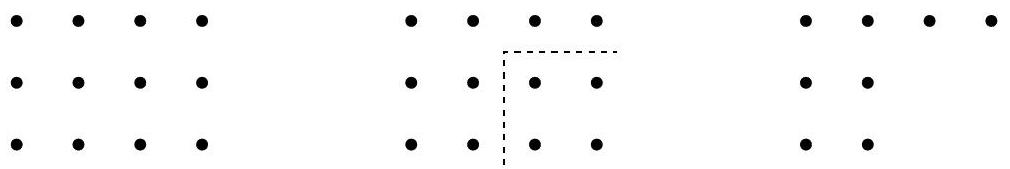
\includegraphics[width=0.85\textwidth]{images/exer-1-5-chomp.jpg}
\end{center}

玩家I是第一个行动的玩家，玩家轮流行动，最后一个移除点的玩家输。

可以把这些点想象成(真正的)饼干:一步行动就是吃掉一块饼干以及它右边和下方的所有饼干，但左上角的饼干是有毒的。

在以下问题中，不要急于套用尼姆值，否则很容易出错。(c)部分有一个巧妙但棘手的答案。

(a) 假设双方都采用最优策略，确定 \(2\times2\)、\(2\times3\)、\(2\times n\) 和 \(m\times m\)(其中 \(m\geq3\)) 巧取游戏中的获胜玩家和制胜行动。证明你的答案。

(b) 如这里所描述的，巧取游戏是一个反常规则的游戏，最后一个行动的玩家输。假设我们想玩同样的游戏，但采用正常规则，即最后一个行动的玩家赢。为了实现这一点，点的阵列应该如何改变？(对于给定的阵列采用正常规则会是一个无聊的游戏，明显的必胜步是取走左上角的点(1,1)。)

(c) 证明任意大小为 \(m \times n\) 的巧取游戏中，先手玩家总能获胜，除非 \(m=n=1\)。[提示:你只需证明存在制胜行动，不必具体指出是哪一步。]
\end{exercise}
\begin{exercise}\label{exer:1.6}
(a) 完成图 1.4 表格中第 5 列和第 6 列、第 0 行到第 3 行的皇后移动博弈等效尼姆堆的条目(假设皇后可以在棋盘上的任意位置)。

(b) 描述图~\ref{fig:1.3} 中皇后移动博弈与尼姆堆之和中的所有制胜行动。
\end{exercise}
\begin{exercise}\label{exer:1.7}
考虑练习~\ref{exer:1.4} 中的塞砖棋游戏，在 \(1 \times  n\) 的棋盘上进行，其中 \(n \geq  2\) 。设 \({D}_{n}\) 为该游戏的尼姆值，使得 \(1 \times  n\) 棋盘的起始位置等效于大小为 \({D}_{n}\) 的尼姆堆。例如， \({D}_{2} = 1\) ，因为 \(1 \times  2\) 棋盘等效于 \(* 1\) 。

(a) 如何从 \(k < n\) 时的较小值 \({D}_{k}\) 计算 \({D}_{n}\) ？[提示:使用博弈之和与 mex 规则。尼姆和的表示法为 \(\oplus\) ，其中当且仅当 \(* a +  * b \equiv   * c\) 时 \(a \oplus  b = c\) 。]

(b) 给出 \({D}_{n}\) 直到 \(n={10}\) 的值。如果你有兴趣，也可以继续算更多项；更大的值会在 \(n={16}\) 时出现，而且序列后来还会重复，只是你可能在发现这一点前已经失去耐心。对于 \(\{1,\ldots,{10}\}\) 中哪些 \(n\)，\(1\times n\) 棋盘上的塞砖棋是必败位置？
\end{exercise}
\begin{exercise}\label{exer:1.8}
考虑在矩形棋盘上进行的以下游戏，每行放置一个白色和一个黑色棋子，例如:(*)

\begin{center}
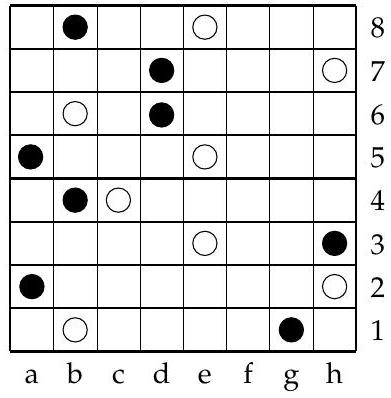
\includegraphics[width=0.45\textwidth]{images/exer-1-8-northcott-start.jpg}
\end{center}

玩家 I 执白并先行动，玩家 II 执黑。两名玩家轮流行动。一次行动中，玩家把自己颜色的某个棋子移动到同一行的其他方格，但不能越过另一枚棋子。例如在上面的 (*) 局面中，第 8 行的白棋可以从 e8 移到 \(\mathrm{c}8,\mathrm{\;d}8,\mathrm{\;f}8,\mathrm{\;g}8\) 或 h8。无法行动的玩家输。

(a) 在以下局面中谁会获胜？

\begin{center}
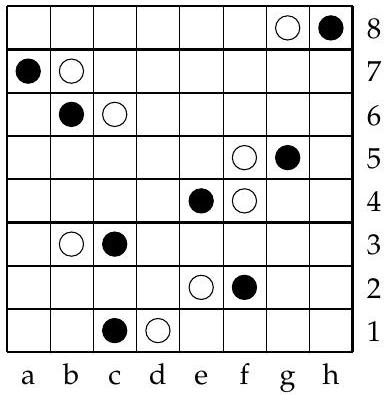
\includegraphics[width=0.45\textwidth]{images/exer-1-8-northcott-position.jpg}
\end{center}

(b) 证明白方在上面的 (*) 局面中可以获胜。给出至少两种制胜行动，并说明理由。[提示:将此游戏与另一个并非无偏、且也违反终止条件的游戏比较；那个游戏仍然接近尼姆游戏，并且若双方走得好，会在有限时间内结束。]
\end{exercise}
\begin{exercise}\label{exer:1.9}
考虑以下网络(用技术术语来说，是一个有向图或“digraph”)。每个圆圈，这里用字母 A 到 P 之一标记，表示网络的一个节点。其中一些节点(这里是 A、F、G、H 和 K)上有棋子。一个节点上可以有任意数量的棋子，例如目前 \(\mathrm{H}\) 上有两个棋子。在一次行动中，其中一个棋子沿着箭头方向移动到相邻节点，例如从 \(\mathrm{F}\) 到 \(\mathrm{I}\) (但不能从 \(\mathrm{F}\) 到 C，也不能直接从 F 到 D)。玩家轮流行动，第一个无法再移动的玩家输。

\begin{center}
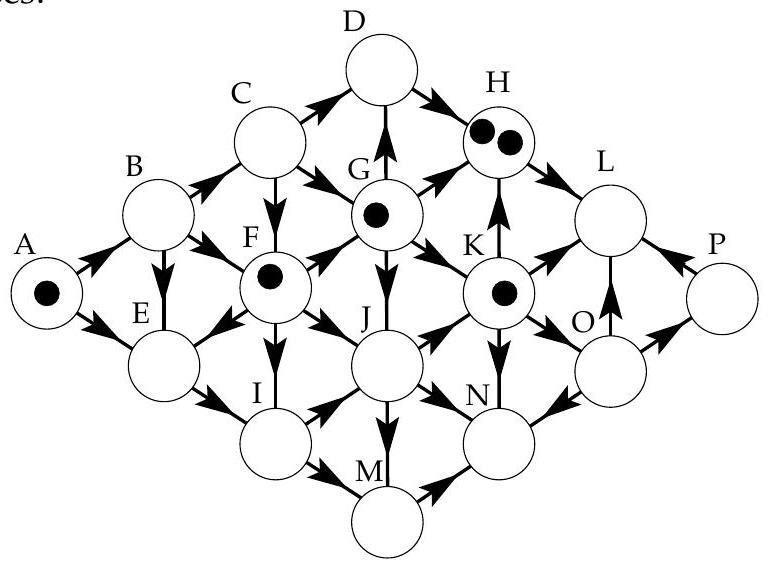
\includegraphics[width=0.60\textwidth]{images/exer-1-9-digraph.jpg}
\end{center}

(a) 解释为什么这个游戏满足终止条件。

(b) 在上述局面中谁会获胜？若先手玩家获胜，描述所有可能的制胜行动。说明你的答案为何正确。

(c) 当从 \(\mathrm{J}\) 到 \(\mathrm{K}\) 的箭头反转，使其从 \(\mathrm{K}\) 指向 \(\mathrm{J}\) 时，(b) 的答案会如何变化？
\end{exercise}
\begin{exercise}\label{exer:1.10}
考虑练习~\ref{exer:1.5} 中大小为 \(2 \times  4\) 的巧取游戏，与大小为 4 的尼姆堆进行博弈之和。

\begin{center}
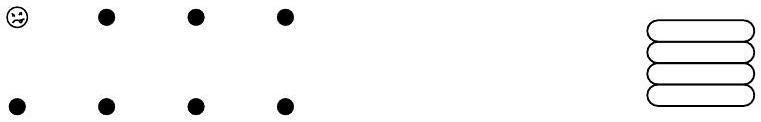
\includegraphics[width=0.75\textwidth]{images/exer-1-10-chomp-nim.jpg}
\end{center}

先手玩家 I 是否有制胜行动？如果有，是哪些？[提示:把巧取游戏(Chomp)改写为正常规则下的博弈(见练习~\ref{exer:1.5}(b)，通过改变点阵实现)，这样输的玩家不是拿到“有毒饼干”的玩家，而是无法继续行动的玩家。这会简化各种尼姆值的计算。]
\end{exercise}

\begin{exercise}\label{exer:1.11}
在 \(m \times  n\) 塞砖棋(Cram)游戏中(见练习~\ref{exer:1.4})，给定一个由 \(m \times  n\) 个方格组成的矩形棋盘。两名玩家交替地将一块多米诺骨牌(domino)水平或垂直放置在两个未被占据的相邻方格上，放置后这两个方格就被占据了。最后能够放置多米诺骨牌的玩家获胜。

(a) 求出 \(2 \times  3\) 塞砖棋的尼姆值，也就是其等价尼姆堆的大小。

(b) 对于一个 \(2 \times  3\) 塞砖棋和一个 \(1 \times  4\) 塞砖棋的博弈之和，如果存在制胜行动，找出全部制胜行动。
\end{exercise}
\begin{exercise}\label{exer:1.12}
考虑尼姆游戏的一个变体，称为分裂尼姆(Split Nim)。它同样使用若干代币堆。玩家可以像普通尼姆游戏那样，从某一堆中取走一些代币；也可以把一个代币堆分裂成两个新的代币堆，两个新堆不必大小相等。例如，大小为 4 的一堆可以减少为 3、2、1 或 0，也可以分裂为大小 1 和 3 的两堆，或大小 2 和 2 的两堆。照常，最后还能行动的玩家获胜。

(a) 分别求出大小为 1、2、3 和 4 的单个分裂尼姆代币堆的尼姆值(等效尼姆堆的大小)。

(b) 分裂尼姆使用局面$(1,2,3)$时，如果存在制胜行动，找出全部制胜行动。

(c) 分裂尼姆使用局面$(1,2,4)$时，如果存在制胜行动，找出全部制胜行动。

(d) 判断以下陈述的真假:“在分裂尼姆游戏中，两个代币堆等效当且仅当它们的大小相等。”证明你的答案。
\end{exercise}
\begin{exercise}\label{exer:1.13}
无偏博弈灰色哈肯布什游戏(Gray Hackenbush)在一个由节点(node)和连接到这些节点或地面的边(edge)组成的图形上进行(地面在下面的图片中用虚线表示)。一次行动是移除一条边，同时移除所有不再与地面相连的边。例如，在下面最左边的图形中，玩家可以移除三根茎中的任何一条边。移除由三条边组成的茎中的第二条边时，会同时移除最上面的边，只留下一条边。所有的边都被涂成灰色，这意味着任何玩家都可以移除它们，所以这是一个无偏博弈。和往常一样，玩家交替行动，最后能够行动的玩家获胜。

(a) 计算以下三个灰色哈肯布什图形的尼姆值(使用你所知道的尼姆游戏和 mex 规则):

\begin{center}
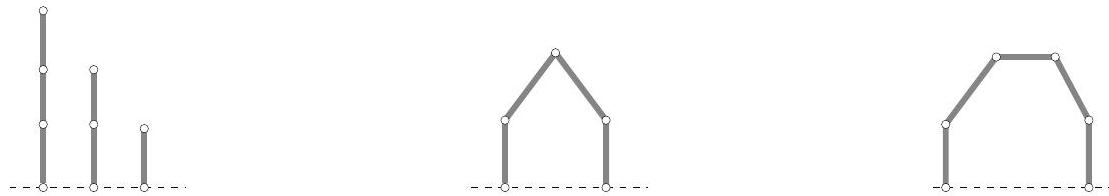
\includegraphics[width=0.75\textwidth]{images/exer-1-13-gray-a.jpg}
\end{center}

(b) 计算以下四个灰色哈肯布什图形的尼姆值:

\begin{center}
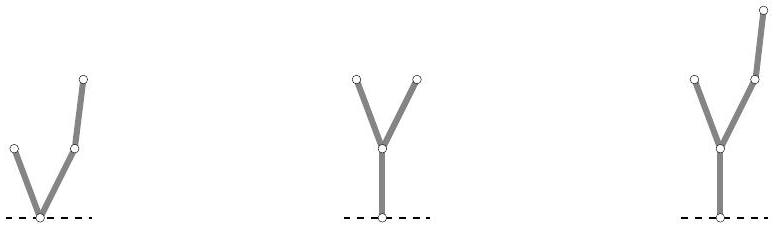
\includegraphics[width=0.75\textwidth]{images/exer-1-13-gray-b.jpg}
\end{center}

(c) 根据 (b) 的答案，给出一个规则来计算一个“树”的尼姆值，这个“树”是通过将几个已知尼姆值的“分支”放在一个大小为 \(n\) 的“茎”上构建的，例如下面图片中的 \(n = 2\) ，其中高度为 3、2 和 4 的三个分支被放在“茎”的顶部。证明该规则的正确性(你可能会发现像 (b) 中那样将分支在底部粘在一起会更有利)。使用这个规则来求出最右边图片的尼姆值。

\begin{center}
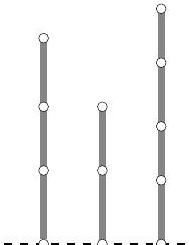
\includegraphics[width=0.75\textwidth]{images/exer-1-13-gray-stems.jpg}
\end{center}

\begin{center}
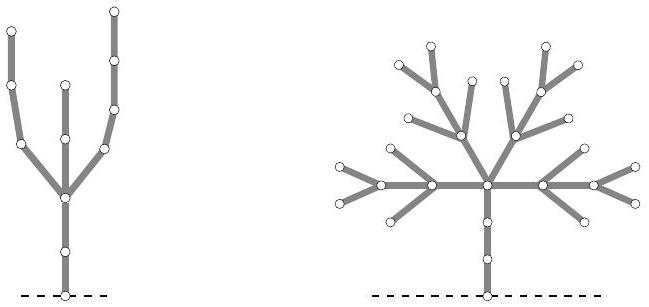
\includegraphics[width=0.75\textwidth]{images/exer-1-13-gray-c.jpg}
\end{center}

\end{exercise}
\begin{exercise}\label{exer:1.14}
本练习是关于第 1.8 节中讨论的有偏博弈(partizan game)。

(a) 通过证明右玩家(Right player)为先手时会输来完成 \eqref{eq:1.32} 的证明。

有偏博弈(黑白)哈肯布什游戏((Black - White) Hackenbush)在一个由节点和连接到这些节点或地面的黑色或白色边组成的图形上进行，如下方图片所示。在一次行动中，左玩家(Left player)移除一条黑色边，右玩家移除一条白色边；如果不存在这样的边，那么该玩家输。在这样的行动之后，所有不再与地面相连的节点和边也会消失。例如，在一个黑色边上面有一条白色边的哈肯布什图形中，左玩家可以移除底部(黑色)边并形成零博弈，而右玩家可以移除顶部(白色)边并留下一条黑色边。

\begin{center}
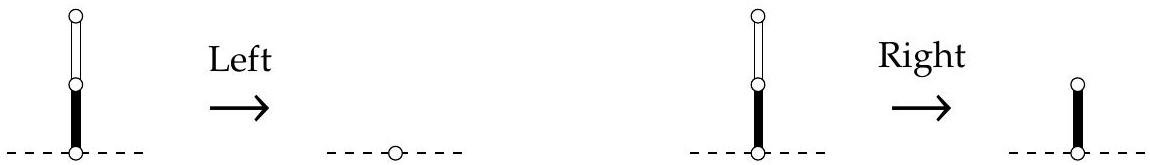
\includegraphics[width=0.50\textwidth]{images/exer-1-14-black-white-example.jpg}
\end{center}

(b) 回顾一下，对于一个组合博弈 \(G\) ，它的负博弈是一个博弈 \(- G\) ，使得 \(G + \left( {-G}\right)  \equiv  0\) 。描述哈肯布什图形的负博弈，并给出一个例子。[提示:参考 \eqref{eq:1.24}。]

我们考虑哈肯布什杆，它们只是由任意一种颜色的边组成的路径。可以证明，任何这样的杆都代表一个数字，这里会考虑一些例子。

(c) 画出表示数字 3 的博弈图(其中先手玩家已经进行了 3 步)。

(d) 找出以下哈肯布什杆所代表的数字。证明你的答案。研究并理解 \eqref{eq:1.36} 会有帮助，并且只考虑玩家的非劣势移动；此外，比较这些博弈中先手(黑色)玩家的实力，以了解答案:
\begin{center}
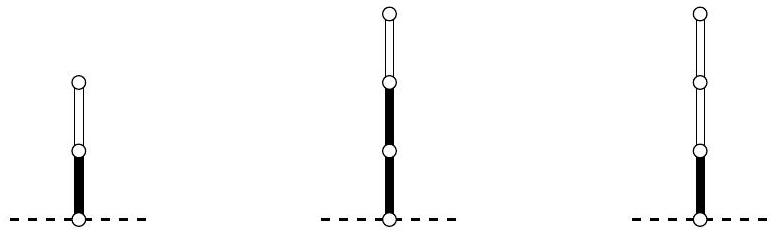
\includegraphics[width=0.70\textwidth]{images/exer-1-14-black-white-rods.jpg}
\end{center}
对于这些博弈，你可以使用以下简写符号:
(e) 构造一个哈肯布什博弈(最好是单个杆)，它代表数字 \(\frac{7}{4}\)。
\end{exercise}

\begin{exercise}\label{exer:1.15}(Albert、Nowakowski 和 Wolfe，2007 年，预备问题 4.1 和 4.2。)

(a) 证明如果 \(G\) 和 \(H\) 是有偏博弈，并且先手玩家在 \(G\) 和 \(H\) 中后手移动时获胜，那么先手玩家在 \(G + H\) 中后手移动时也获胜。[提示:用结果类来表示先手玩家后手移动获胜的含义，如 \eqref{eq:1.31} 所示。]

(b) 给出博弈 \(G\) 和 \(H\) 的一个例子，使得先手玩家在 \(G\) 和 \(H\) 中先手移动时获胜，但在先手玩家可以选择在博弈之和 \(G + H\) 中先手或后手移动的情况下，也无法在 \(G + H\) 中获胜。[提示:这两个博弈都能是数字博弈吗？或者是无偏博弈吗？] 2

\end{exercise}
